\documentclass[UTF-8,a4paper,zihao=-4]{ctexart}
\usepackage[a4paper,left=3cm,right=2.5cm,top=3cm,bottom=2.5cm]{geometry}
\usepackage{graphicx} % Required for inserting images
\usepackage[backend=biber,style=gb7714-2015]{biblatex} 
\usepackage[labelfont=bf,textfont=bf]{caption}
\addbibresource{ref.bib} %待补上参考文献 
\usepackage{amsmath,amssymb}   % 公式
\usepackage{graphicx}          % 插图
\usepackage{booktabs}           % 三线表
\usepackage{hyperref}           % 超链接（最后加载，少数例外）
\usepackage{placeins}
\usepackage{subcaption}
\usepackage{csvsimple}
\usepackage{listings}
\usepackage{xcolor}
\usepackage{float}
\pagestyle{plain} 
\ctexset{
  section = {
    number = \chinese{section},   % 中文数字：一、二、三…
    format = \zihao{3}\heiti\centering,
    aftername = \quad,            % 编号和标题之间的空格（可调）
    % 如果你想变成“一、绪论”（带顿号），把 aftername 改成 \hspace{1em} 或直接写顿号
  }
}
\makeatletter
\renewcommand{\maketitle}{
    \begin{center}
        \vspace*{-2cm}
        {\zihao{2}\heiti\@title\par}
    \end{center}
}
\makeatother

\makeatletter
\renewenvironment{abstract}
{
    \begin{center}
        {\zihao{-3}\textbf{摘要}}
    \end{center}
    \zihao{-4}
}
{}
\makeatother

\lstset{
    language=Python,
    basicstyle=\ttfamily\small,
    numbers=left,
    numberstyle=\tiny,
    frame=single,
    breaklines=true,
    columns=fullflexible
}

\begin{document}

\title{复杂工况下巷道锚杆预紧力矩的建模与分析}
\date{}
\maketitle

\begin{abstract}

    \textbf{针对问题一：}针对问题1.1，直接对给出的理想实验数据进行\textbf{最小二乘拟合}，得到预紧力矩T与预紧力P之间的正比例关系，通过得到的直线斜率计算扭矩系数K在锚杆直径18mm，20mm，22mm下的值分别为\textbf{0.1620,0.1831，0.1899}。针对问题1.2，对于工况实测数据的临界点判断是\textbf{断点分析问题}，本文采用\textbf{分段回归与扭矩系数变异系数$CV_K$相结合的方法}进行判断，对于所有可选临界点中寻找决定系数$R^2$大于0.99，扭矩系数变异系数$CV_K$发生显著变化后趋于稳定的点为临界点，最后确定在\textbf{岩石工况}下力矩临界点为\textbf{125N·m}，在\textbf{煤体工况}下力矩临界点为\textbf{175N·m}。

    \textbf{针对问题二：}针对问题2.1，依据附录二的三个约束，按照仅使用托盘和可以使用钢带两种情况进行分类讨论，然后将允许最大预紧力矩$T_{max}$的建模为优化问题的求解，并解出最终的通用参数模型,并依据围岩压陷极限的约束讨论了钢带使用的必要性。针对问题2.2，将问题一求得的扭矩系数K和表四的数据代入到问题2.1建立的模型中进行求解，解得在工况A：岩层锚杆中，\textbf{最大允许预紧力矩$T_{max}=$726.24{N$\cdot$m}，不需要钢带}，在工况B：煤层锚杆中，\textbf{仅使用托盘时最大允许预紧力矩$T_{max}=$843.938N$\cdot$m}；\textbf{可以使用钢带时最大允许预紧力矩$T_{max}=$1163.263N$\cdot$m}。\textbf{需要使用钢带}。

    \textbf{针对问题三：}针对问题3.1，我们结合附录三的三个应力的叠加以及附录一的符号说明进行推导，按照材料许用应力的约束进行公式整理，计算出偏心受力状态下最大允许预紧力矩$T_{max}$与偏心距e关系的数学模型。然后从其计算方式，公式严谨性和现实工程情况角度分析其适用性与局限性。针对问题3.2，我们依照有偏心距的情况对问题二的三个约束进行修正，并得到最终的考虑多种失效的模型。

    \textbf{针对问题四：}

\noindent \textbf{关键词：}
\end{abstract}

\newpage
\section{问题背景与重述}
\subsection{问题背景}
巷道围岩支护是防止顶板垮塌，保障设备正常运行，保证矿井高效安全生产的重要手段。 而在众多防护手段中，锚杆支护展现出了强大的优势，其支护原理是通过拧紧锚杆尾端螺母，施加预紧力矩，经由螺纹传动转化为沿杆体轴向的预紧力，进而使围岩由二向受力状态转化为三向受力状态，从而实现主动支护。

在工程中，一般认为预紧力矩越大预紧力越大，且支护效果越好，但实际探究发现，预紧力矩与预紧力并非完全的线性关系，并且还受多种因素影响，因此为了更高效、更科学的配置使用锚杆支护，有必要深入研究预紧力矩与预紧力的转换机制，为此我们将从下面四个问题进行探究。
\subsection{问题要求}
\begin{enumerate}
    \item 在标准实验条件下，锚杆预紧力矩 T 与预紧力 P 通常可近似表示为线性关系$T=K\cdot P\cdot d$，其中 d 为锚杆直径，K 为扭矩系数。但在实际加载初期，受螺纹间隙、垫圈变形及接触面压实等因素影响，二者往往表现出较强的非线性；当预紧力矩超过某一临界值后，系统才逐渐进入稳定的线性工作阶段。

    因此，我们需要利用附件表1中的实验数据建立不同直径锚杆的预紧力矩—预紧力关系数学模型，并计算相应的扭矩系数 K；此外需要进一步结合表2和表3中直径为20 mm锚杆的实测数据，给出由非线性阶段转入线性阶段的临界预紧力矩。
    
    \item 当预紧力过小时，锚杆难以发挥有效支护作用；当预紧力过大时，则可能引起锚杆屈服、锚固界面破坏或托盘压入围岩，而钢带可扩大受力面积，从而降低松软围岩发生局部压陷的风险。
    
    因此，我们需要依据附录2给出的力学关系和工程约束，建立最大允许预紧力矩$T_{max}$的通用参数化模型，并给出是否需要使用钢带的判定条件；并在此基础上，利用附件表4中的参数分别计算工况A和工况B下的$T_{max}$，并判断两种工况是否需要增设钢带。
    
    \item 受煤岩体破碎和钻孔不规则等因素影响，锚杆轴线与围岩表面法线之间可能存在偏心距 e。此时，轴向预紧力会产生附加弯矩，使锚杆螺纹段同时承受拉伸、弯曲和扭转作用，从而增加螺纹根部发生断裂的风险。
    
    因此，我们需要根据附录3建立偏心条件下$T_{max}$与 e 的数学模型，并分析名义截面模型的适用范围及局限性；同时，我们还应将偏心受力与附录2中的锚杆强度、锚固能力和围岩压陷等约束结合，分析偏心距e是否会影响约束的有效性，构建综合多种失效模式的修正模型，给出$T_{max}(e)$的表达式并进行数值验证。
    
    \item 不同围岩的力学性质差异较大。松软围岩承载能力较低，过大的预紧力容易引起压陷或破坏；坚硬围岩则能够承受更高的支护荷载。若统一采用相同的施工力矩，可能同时造成软岩中过载和硬岩中支护能力利用不足的问题。
    
    因此，我们需要以普氏系数 f 表示围岩坚固程度，结合各类失效约束，建立最优预紧力矩$T_{opt}$与f关系的数学模型；此外，还需判断不同围岩区间内的最先限制预紧力矩的主控失效模式，并对模型的有效性和可靠性进行检验。
    
\end{enumerate}

\section{问题分析}
\subsection{问题一分析}
附件中表1给出的是标准实验数据，所以此时预紧力矩T与预紧力P之间满足正比例关系，只需要对所给的数据进行最小二乘拟合，根据得到斜率即可求得扭矩系数K。而表2表3是在实际工况下测得的数据，二者并非始终线性相关，需要寻找临界点。因此该问题本质是对数据的断点分析，但是直接对两段数据点进行拟合需要考虑非线性部分具体的拟合函数，如果强制使用某个函数从纯数据角度进行拟合，既忽略了数据代表的实际物理工程含义，也有可能出现过拟合现象。因此本文从稳定工作状态下二者保持稳定线性关系的角度出发，通过计算扭矩系数变异系数$CV_K$的变化曲线，选择$CV_K$发生显著变化后开始保持稳定的点作为临界点。

\subsection{问题二分析}
附录二中已经给出了相关物理模型与工程约束条件“锚杆强度极限”、“锚固系统极限”，而问题一已经给出了预紧力矩与预紧力的数学模型，故我们便可在此基础上建立最大允许预紧力矩$T_{max}$的通用参数化模型，并根据约束条件(3)“围岩压陷极限”，进一步分类讨论具体的通用参数化模型，同时其也是使用钢带的判定条件。在建立好$T_{max}$的通用参数化模型后，便可结合具体参数来计算工况A、B的$T_{max}$并判断是否需要增设钢带。

\subsection{问题三分析}
附录三中已经给出了偏心条件下相关的力学公式，我们可以依此进行数学推导并建立起对应的数学模型，同时根据力学公式以及推导过程中作出的一些前提假设，来进行对名义截面模型的分析；在分析完后可根据模型来分析偏心距e的影响，至于多种失效模式的修正模型，则可以结合问题二所建数学模型，进行总结修正，并带入数值进行验证。

\subsection{问题四分析}
附录中并没有明确给出普氏系数f与$T_{opt}$的关系式，但指出了f与单轴抗压强度有关，我们可以查阅相关资料，找到单轴抗压强度与其他相关参数（如弹性模量E）的关系，并以此进一步推导建立联系，最终构建起$T_{opt}$与f的数学模型，并以此进行判断不同围岩条件下的主控失效模式，以及对模型进行有效性验证和可靠性验证。

%%%%%准备工作%%%%%
\section{初步准备}
\subsection{模型假设}
\begin{enumerate}
    \item 假设同一力矩下的5个测点具有相同代表性，可以求取平均值表示该力矩下的总体预紧力。
    \item 模型对应的围岩主要为单一主体，即分析某类围岩时认为其杂质较少，可以认为杂质不影响围岩主要性质。
    \item 在锚杆材料、表面状态等基本一致的条件下，实际工况相对于标准实验条件对扭矩系数产生的影响可表示为近似不变的修正系数。
    \item 
    \item 
\end{enumerate}

%%表%%
\subsection{符号说明}
本文所使用的符号及说明如下表所示。
\begin{table}[H]
\centering
\zihao{5}

\caption{符号说明}
\begin{tabular}{ccc}
\toprule
符号 & 说明 & 单位 \\
\midrule
$T$ & 预紧力矩 & $N\cdot m$ \\
$P$ & 预紧力 & kN \\
$d$ & 锚杆直径 & mm \\
$K$ & 扭矩系数\\
$R^2$ & 决定系数\\
$CV_K$ & 扭矩系数变异系数\\
\bottomrule
\end{tabular}

\vspace{0.5em}
\parbox{0.9\textwidth}{
\zihao{5}
注：其他符号已在相应部分中说明。
}
\end{table}

%%%%%模型建立与求解%%%%%
\section{模型建立与求解}
\subsection{问题一的模型建立与求解}
\subsubsection{问题1.1的建模与求解}
由于表1提供的数据是标准实验数据，说明这是在在材质均匀、界面平整的标准实验条件下得到的数据，我们可以认为预紧力矩与预紧力呈正比例关系，用工程中常用的公式表示，即

\begin{equation}
T=KPd
\label{TandP}
\end{equation}
对同一直径的锚杆而言，$d$ 为常数，因此可将上式写成

\begin{equation}
T=aP,\qquad a=Kd
\end{equation}
因此本题需要建立的预紧力矩与预紧力之间的数学模型就是通过实验数据采用过原点的最小二乘法拟合 $T$ 与 $P$ 的正比例关系，目标函数为

\begin{equation}
S(a)=\sum_{i=1}^{7}(T_i-aP_i)^2
\end{equation}
对 $a$ 求偏导并令其为零，有

\begin{equation}
\frac{\partial S(a)}{\partial a}
=-2\sum_{i=1}^{7}P_i(T_i-aP_i)=0
\end{equation}
因此斜率估计值为

\begin{equation}
a=\frac{\sum_{i=1}^{7}P_iT_i}{\sum_{i=1}^{7}P_i^2}
\end{equation}
同时为了评价拟合效果，计算决定系数

\begin{equation}
R^2=1-\frac{\sum_{i=1}^{7}(T_i-\hat{T}_i)^2}
{\sum_{i=1}^{7}(T_i-\bar{T})^2}
\end{equation}
对$d$=18mm,20mm,22mm依次用该方法拟合得到如下图像：

\begin{figure}[H]
\centering
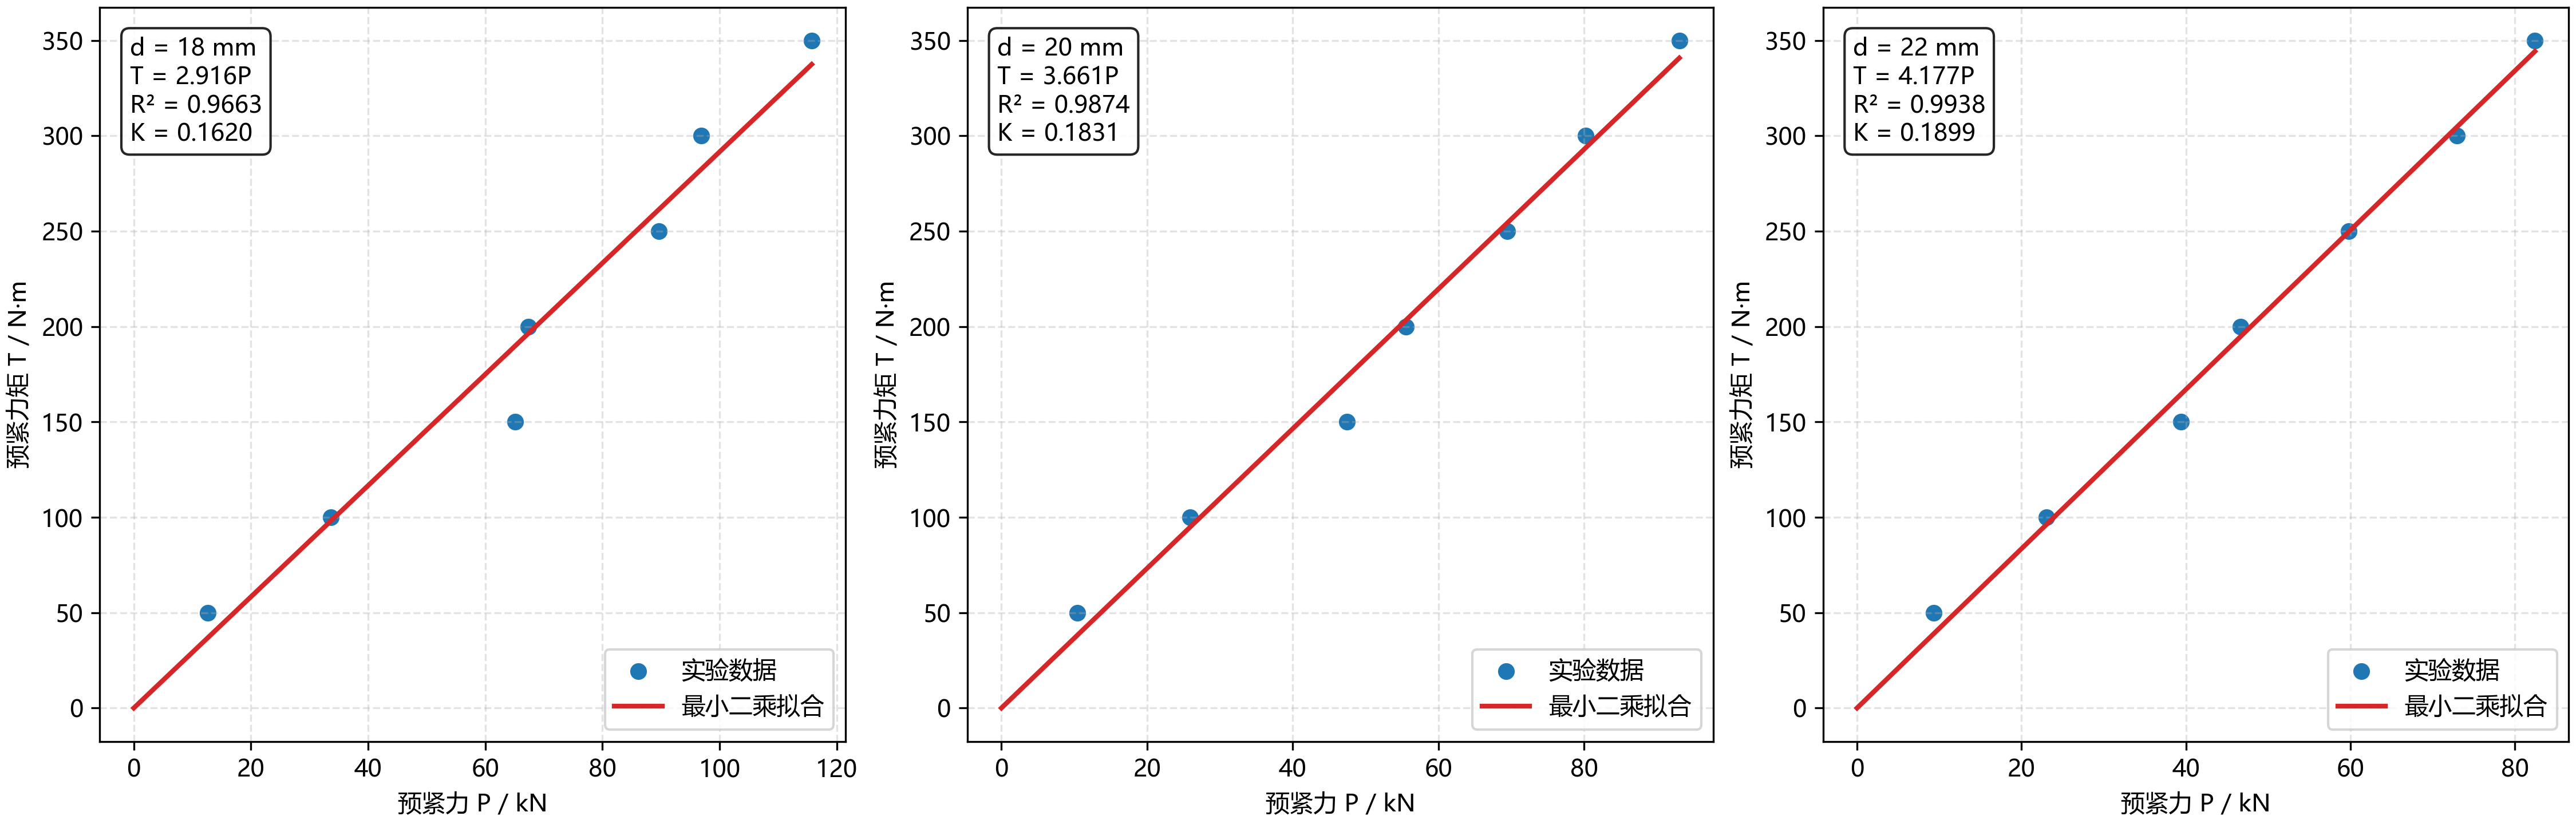
\includegraphics[width=1.00\textwidth]{outputs/figures/question1_1_linear_fit.png}
\caption{不同直径预紧力矩与预紧力拟合关系}
\end{figure}

从图中可以明显看出，两者对正比例关系的拟合效果较好，在$d$=18mm,20mm,22mm不同直径下的决定系数分别达到了0.9663,0.9874,0.9938，证明了直线拟合的准确性。此时，计算得到的扭矩系数K为\textbf{0.1620,0.1831，0.1899}。

从标准实验下的结果可以看出，随着直径$d$的增大，我们对拟合直线的决定系数越来越大，拟合效果越来越好，扭矩系数K越来越大。说明直径$d$的变化会影响线性关系的拟合效果和K值，是后续问题解答过程中需要注意的问题。

\subsubsection{问题1.2实际工况下断点分析模型的建立}
表2和表3提供的数据是对于真实岩石与煤体工况下的实测数据，与标准实验条件不同，在加载初期，存在螺纹间隙、垫圈变形及接触面压实过程的影响，因此不能整过程拟合为正比例直线，而需要分成非线性和线性关系两部分研究。因此寻找临界力矩，就是要找出由非线性关系转入线性关系的临界点，所以本文将该问题看作断点回归问题。设候选临界预紧力矩为 $T_c$，当 $T_i\geq T_c$ 时，认为数据进入稳定线性阶段。

由于在实测数据中每一个力矩下有5个测点，为降低局部测量误差的影响，先对同一力矩等级下的5个预紧力测点取平均。设第 $i$ 个力矩等级为 $T_i$，对应5个测点预紧力为 $P_{i1},P_{i2},\cdots,P_{i5}$，则平均预紧力为

\begin{equation}
\bar{P}_i=\frac{1}{5}\sum_{j=1}^{5}P_{ij}
\end{equation}

在候选临界点之后，就可以采用过原点的正比例模型进行拟合，
\begin{equation}
T=aP
\end{equation}
但是前半部分的非线性部分由于离散型较大，对于分几段拟合，用什么函数拟合很难确定，并且这一段模型的选择也会很大程度上影响最终临界点的选择，所以我们放弃对整段数据用一个全局的分段函数进行拟合建模，而是仅对临界点之后的线性部分使用正比例模型建模，避免了非线性部分拟合不当对临界点选择的影响。

同时，本问题由于具有鲜明的工程物理的实际意义，仅从数据回归的角度选择临界点会导致过拟合的现象出现，同时抛弃了数据本身具有的物理意义。因此在使用分段回归方法的基础上，我们又引入了扭矩系数变异系数$CV_K$来评价临界点之后点的预紧力矩，预紧力测量过程的重复性、一致性和稳定性\cite{tran2026nut}，表示对于公式$T=KPd$的贴合效果，当选择 $T_c$ 为候选临界点时，仅保留 $T_i\geq T_c$ 的后段数据。设后段共有 $m$ 个等效扭矩系数 $K_1,K_2,\cdots,K_m$，则后段平均扭矩系数为

\begin{equation}
\bar{K}(T_c)=\frac{1}{m}\sum_{T_i\geq T_c}K_i
\end{equation}
样本标准差为

\begin{equation}
s_K(T_c)=
\sqrt{
\frac{1}{m-1}
\sum_{T_i\geq T_c}
\left[K_i-\bar{K}(T_c)\right]^2
}
\end{equation}
于是等效扭矩系数变异系数为\cite{GBT1231_2024}

\begin{equation}
CV_K(T_c)=\frac{s_K(T_c)}{\bar{K}(T_c)}\times 100\%
\end{equation}

同时计算$R^2$ 用于反映后段线性拟合程度，配合$CV_K$ 反映后段等效扭矩系数的离散程度。若随着截断起始力矩增大，在某个力矩处满足$R^2\geq0.99$，且$CV_K$ 出现显著变化并在后续保持稳定时，我们就认为数据在该处由压实阶段进入了稳定工作状态，可以认为该力矩值为临界力矩。
\subsubsection{问题1.2临界点求解过程}
根据上述思路，分别对岩石工况和煤体工况进行逐点的截断分析。先对同一预紧力矩下的5个测点取平均，得到每个力矩等级对应的平均预紧力 $\bar{P}_i$。然后以每一个力矩等级作为候选临界点，仅保留该点及其之后的数据，采用过原点最小二乘法拟合 $T=aP$并计算该候选截断点下的决定系数 $R^2$ 与等效扭矩系数变异系数 $CV_K$。最后，绘制 $R^2$ 和 $CV_K$ 随截断起始力矩变化的曲线如下。

对岩石工况：
\begin{figure}[H]
\centering
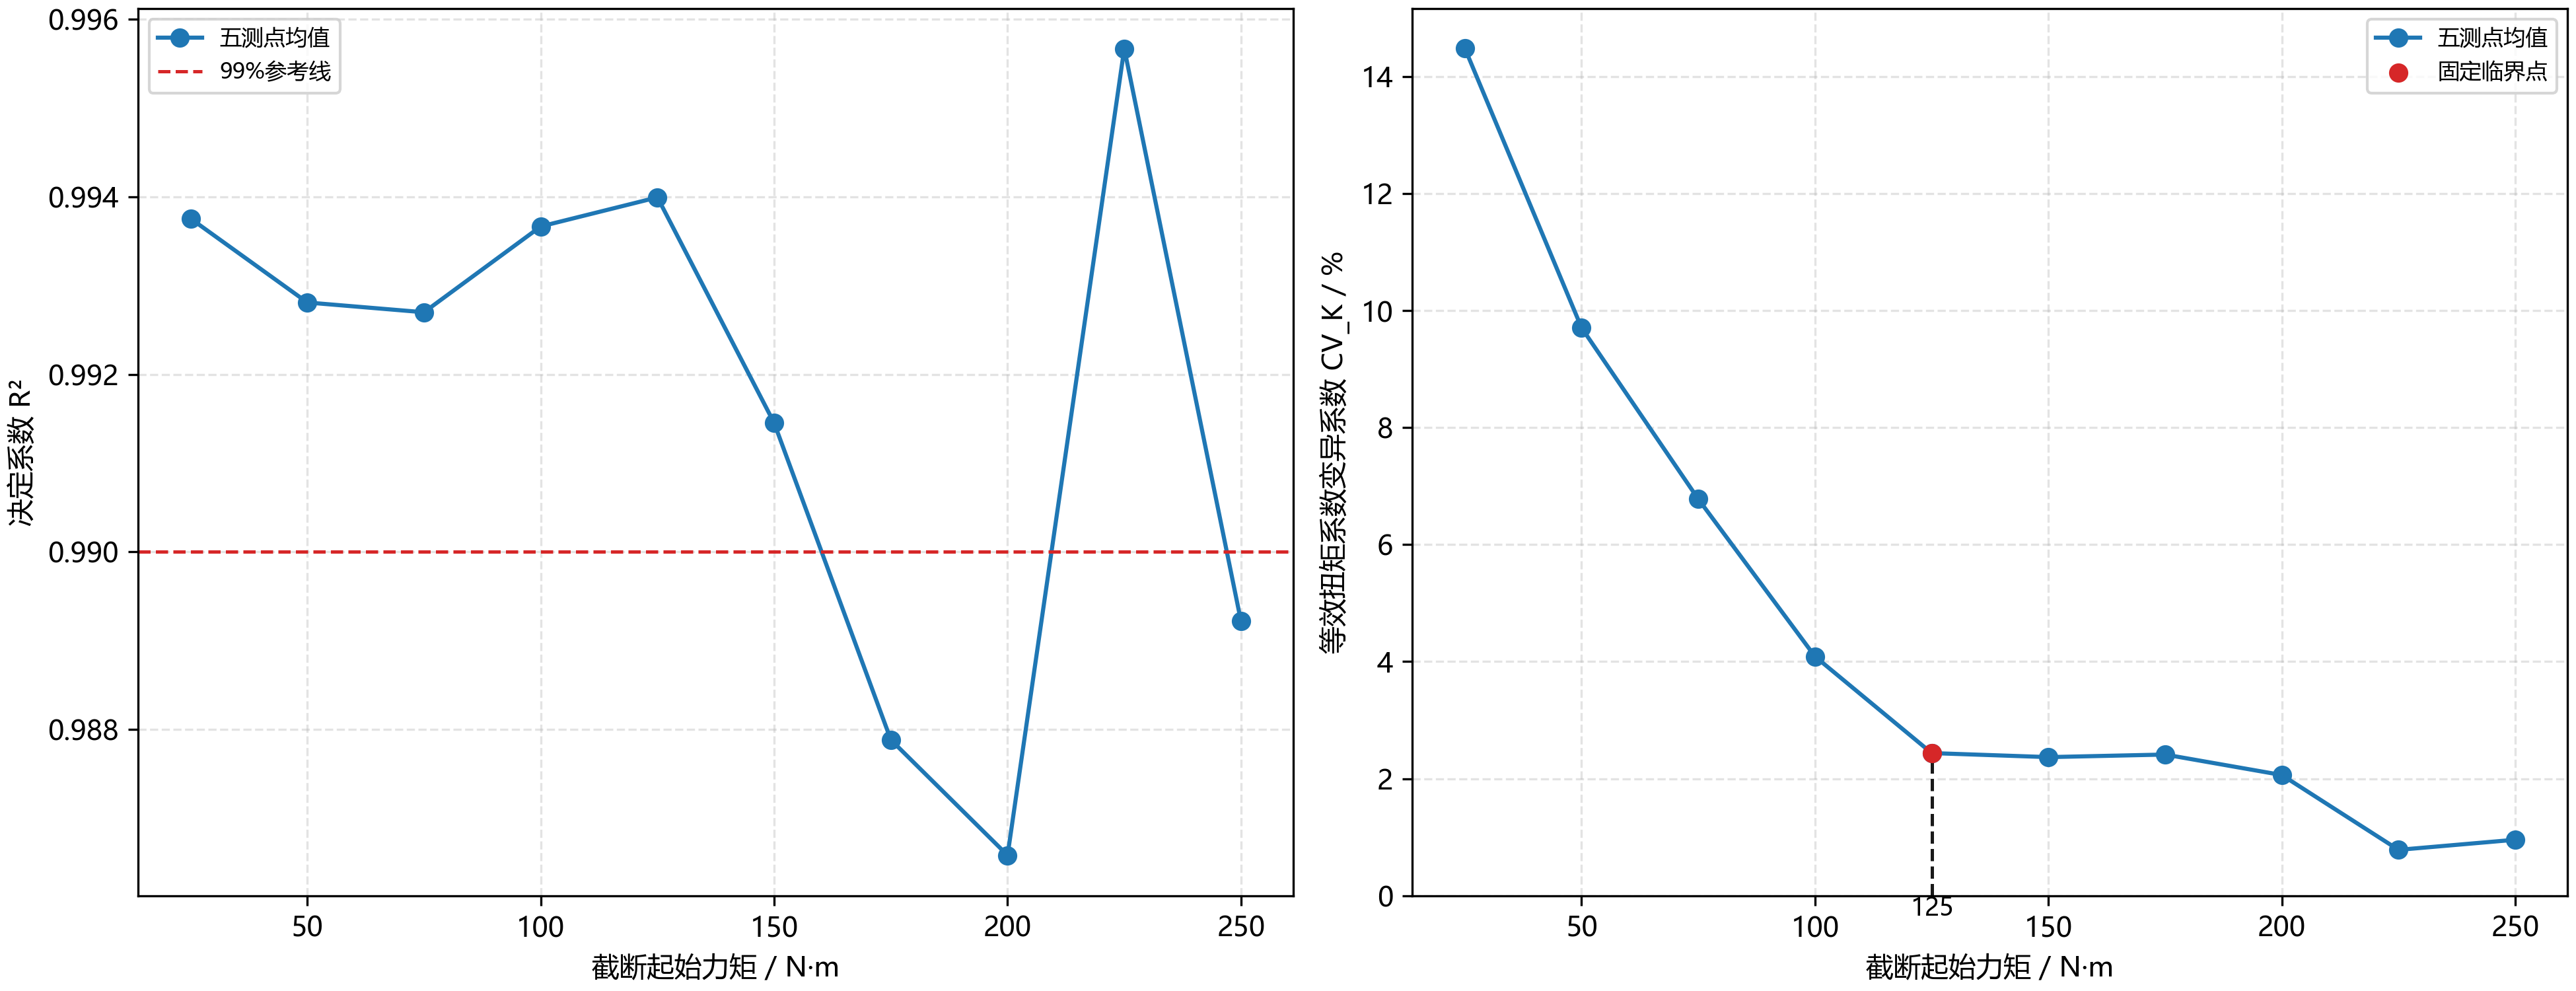
\includegraphics[width=0.9\textwidth]{outputs/figures/question1_2_rock_r2_cv_k.png}
\caption{岩石工况下$R^2$与$CV_K$随临界力矩变化曲线}
\end{figure}
发现决定系数在临界力矩150之前一直保持在0.99以上，同时扭矩系数变异系数$CV_K$在前期呈现明显下降趋势并在$125$N·m开始逐渐保持平稳，因此我们认为数据在数据在$125$N·m之后预紧力矩和预紧力就有明显且良好的线性关系，因此选择\textbf{125N·m}作为临界力矩。

对煤体工况：
\begin{figure}[H]
\centering
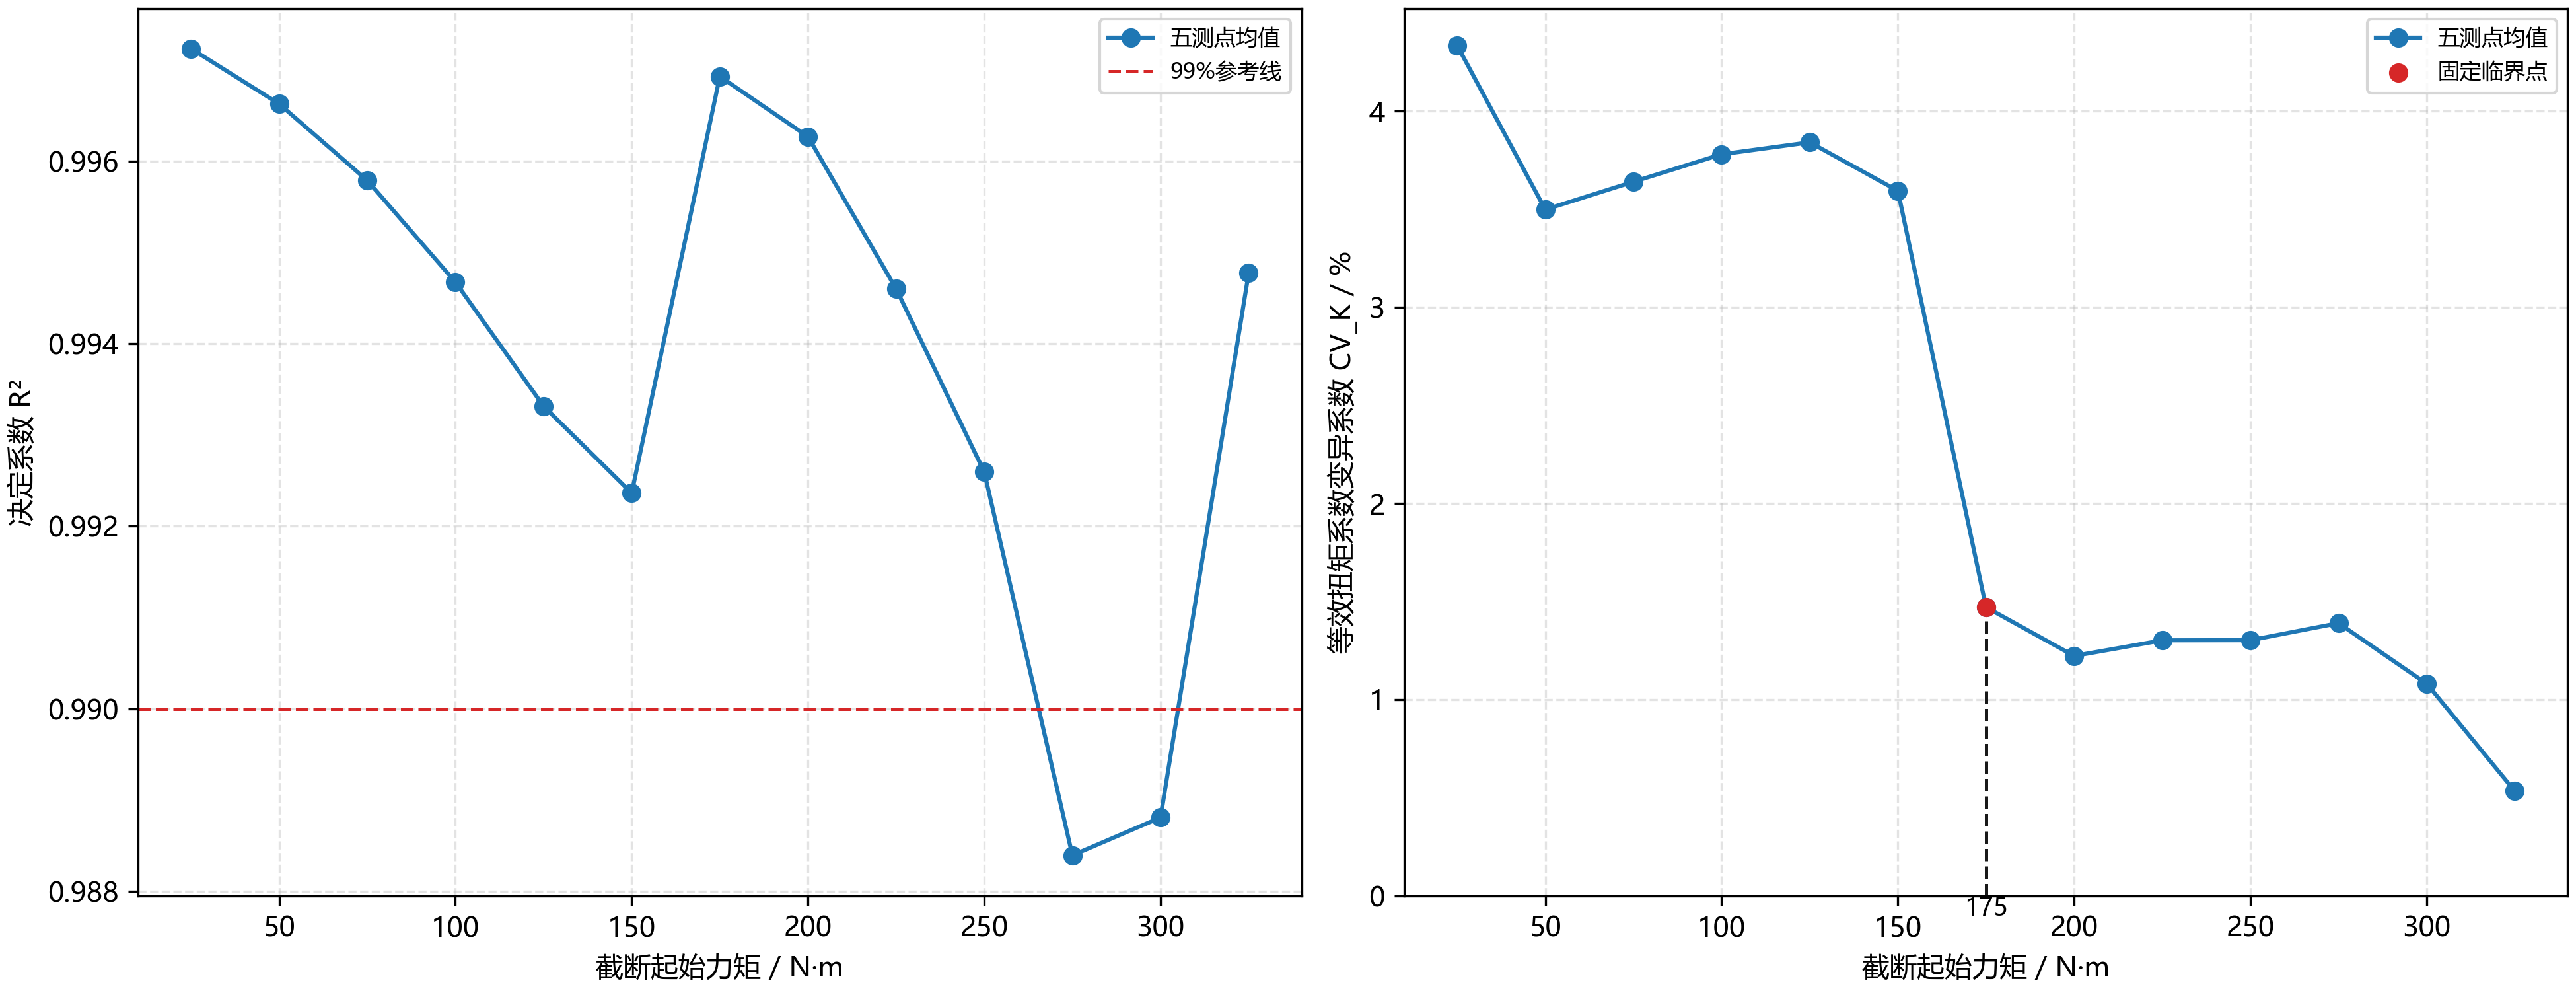
\includegraphics[width=0.9\textwidth]{outputs/figures/question1_2_coal_r2_cv_k.png}
\caption{煤体工况下$R^2$与$CV_K$随临界力矩变化曲线}
\end{figure}
发现决定系数在临界力矩250之前一直保持在0.99以上，同时扭矩系数变异系数$CV_K$在$175$N·m处有明显下降趋势，后续开始逐渐保持平稳，因此我们认为数据在数据在$175$N·m之后预紧力矩和预紧力就有明显且良好的线性关系，因此选择\textbf{175N·m}作为临界力矩。
\subsubsection{问题1.2模型的验证与工程合理性分析}
为检验所选临界力矩的合理性，本文进一步绘制了临界力矩后数据的拟合直线并计算了残差分布，由于最终模型为
\begin{equation}
T=aP
\end{equation}
因此在给定力矩 $T_i$ 下，模型得到的预紧力为
\begin{equation}
\hat{P}_i=\frac{T_i}{a}
\end{equation}
因此残差定义为
\begin{equation}
e_i=P_i-\hat{P}_i
\end{equation}
如果所绘直线拟合较好，残差均匀分布在零残差周围且没有明显单调趋势，我们就认为所选临界力矩正确。

对岩石工况，得到拟合直线与残差如下：
\begin{figure}[H]
\centering
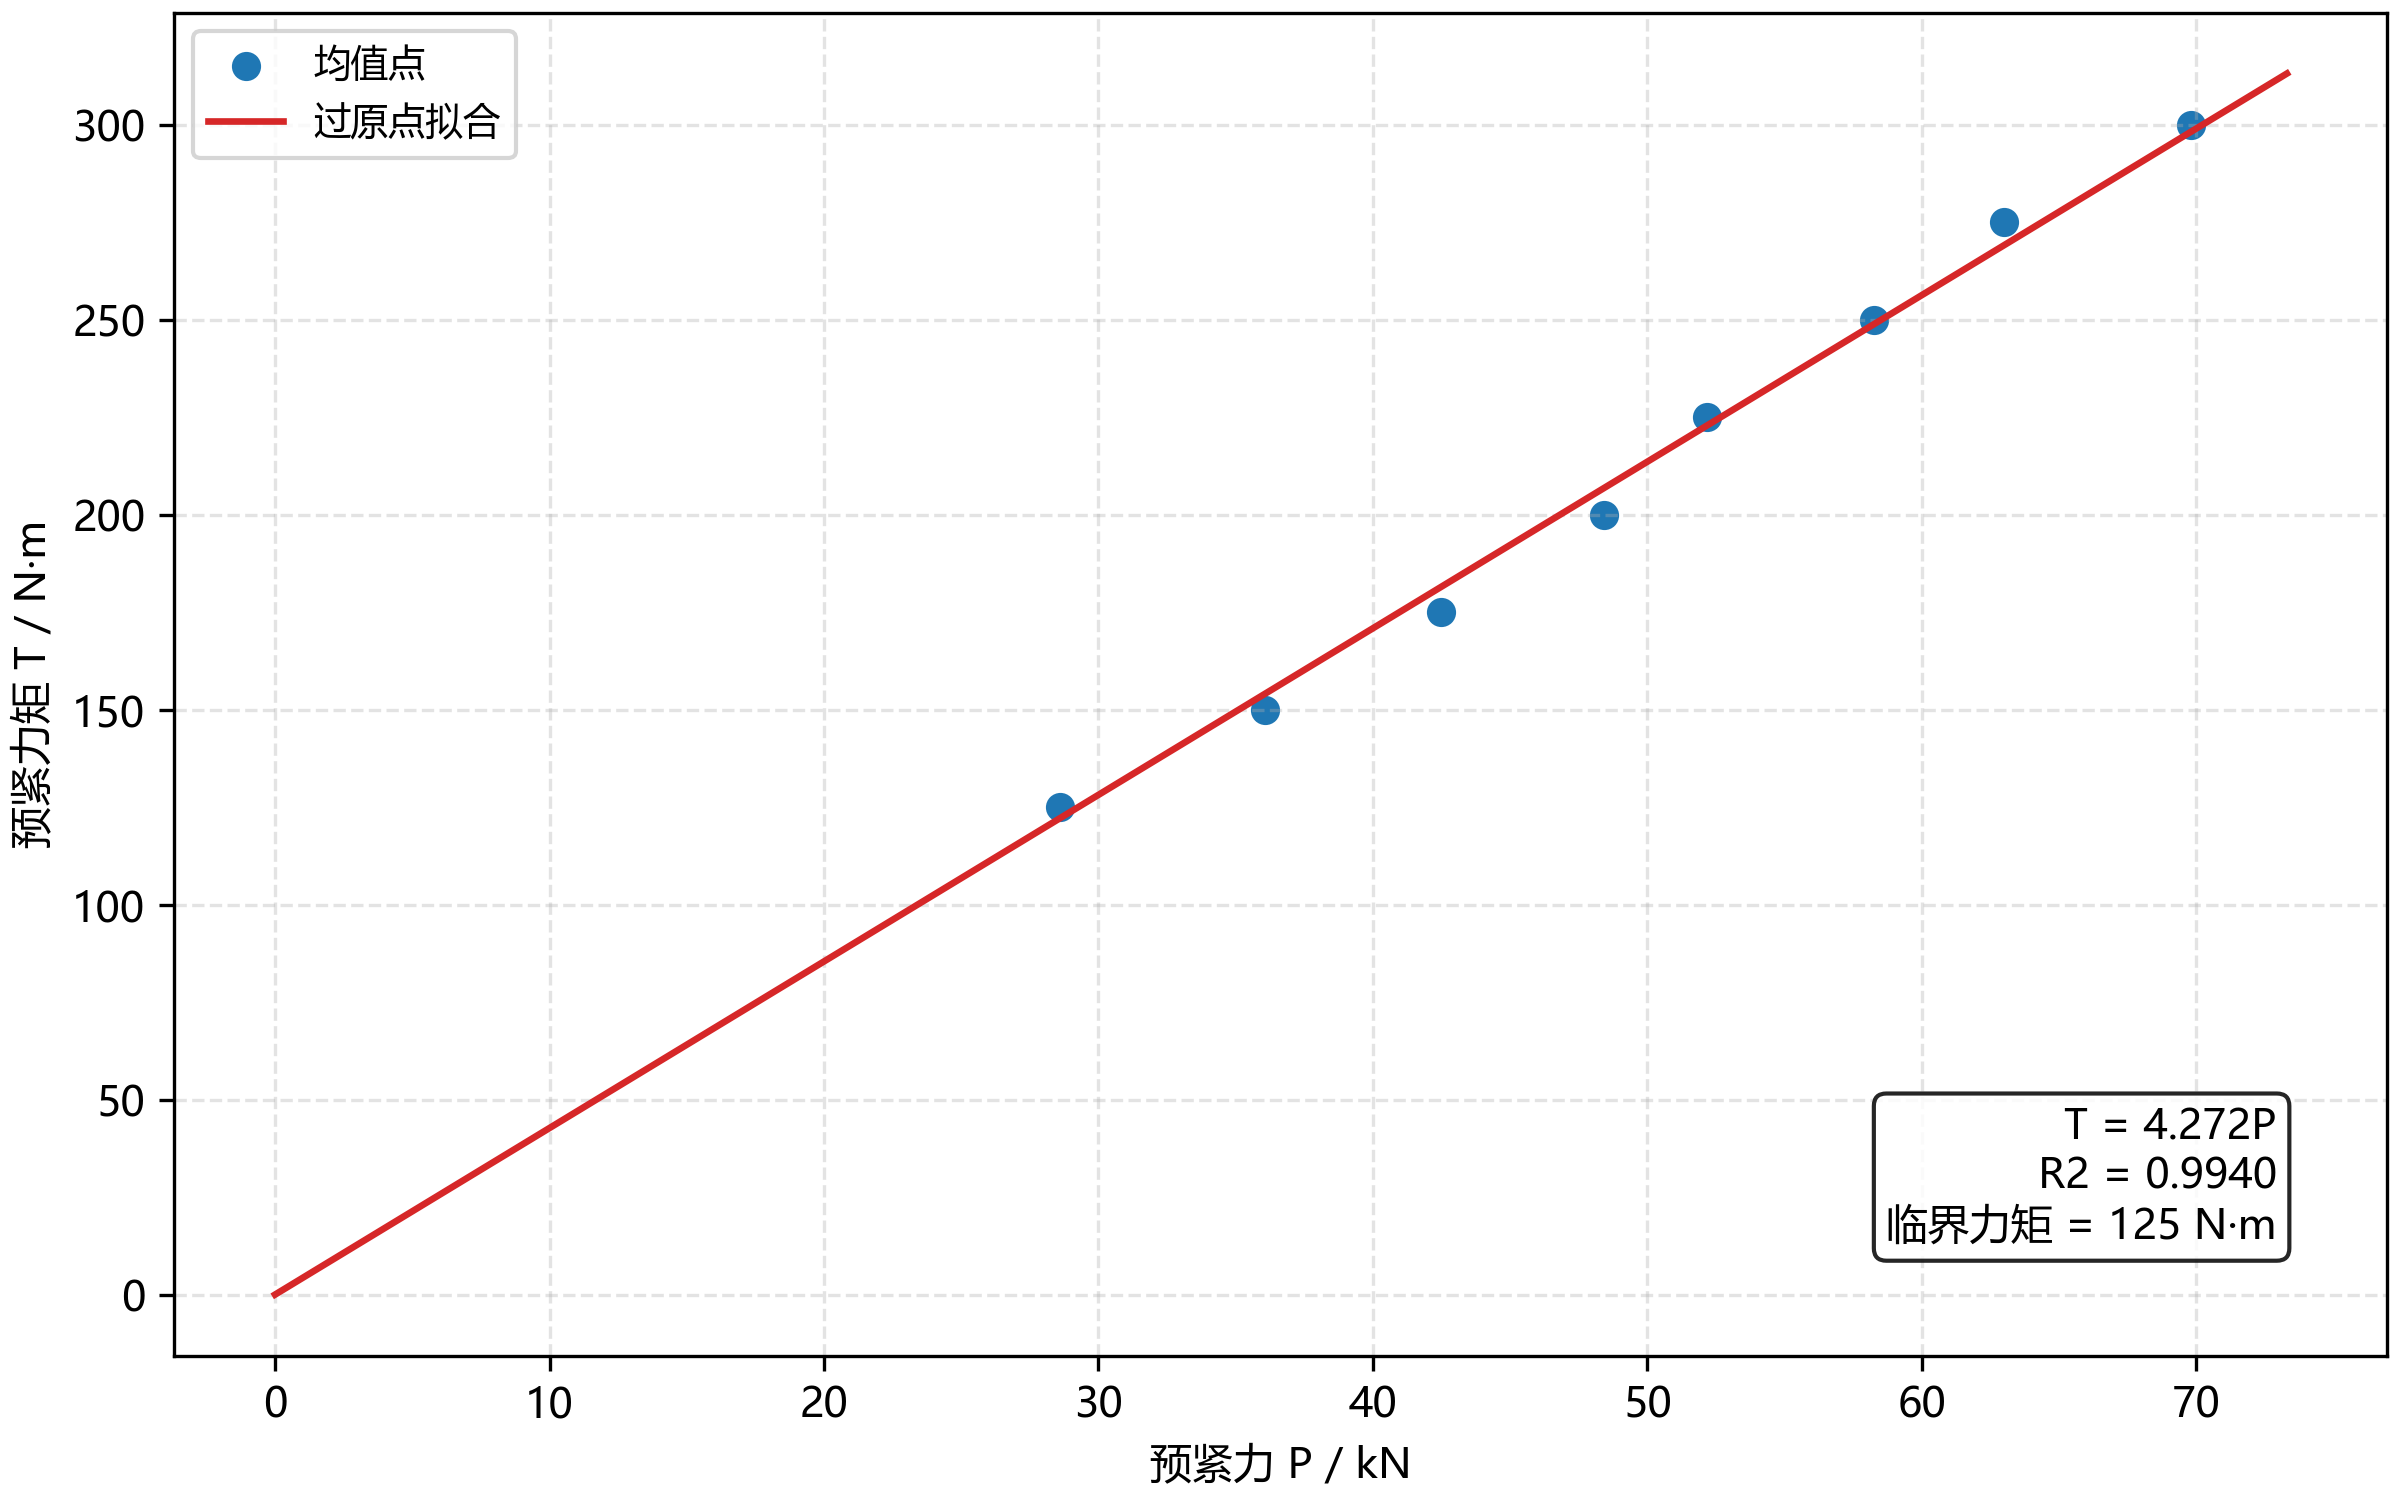
\includegraphics[width=0.85\textwidth]{outputs/figures/question1_2_rock_fixed_fit.png}
\caption{岩石工况临界点后数据拟合结果}
\end{figure}
\begin{figure}[H]
\centering
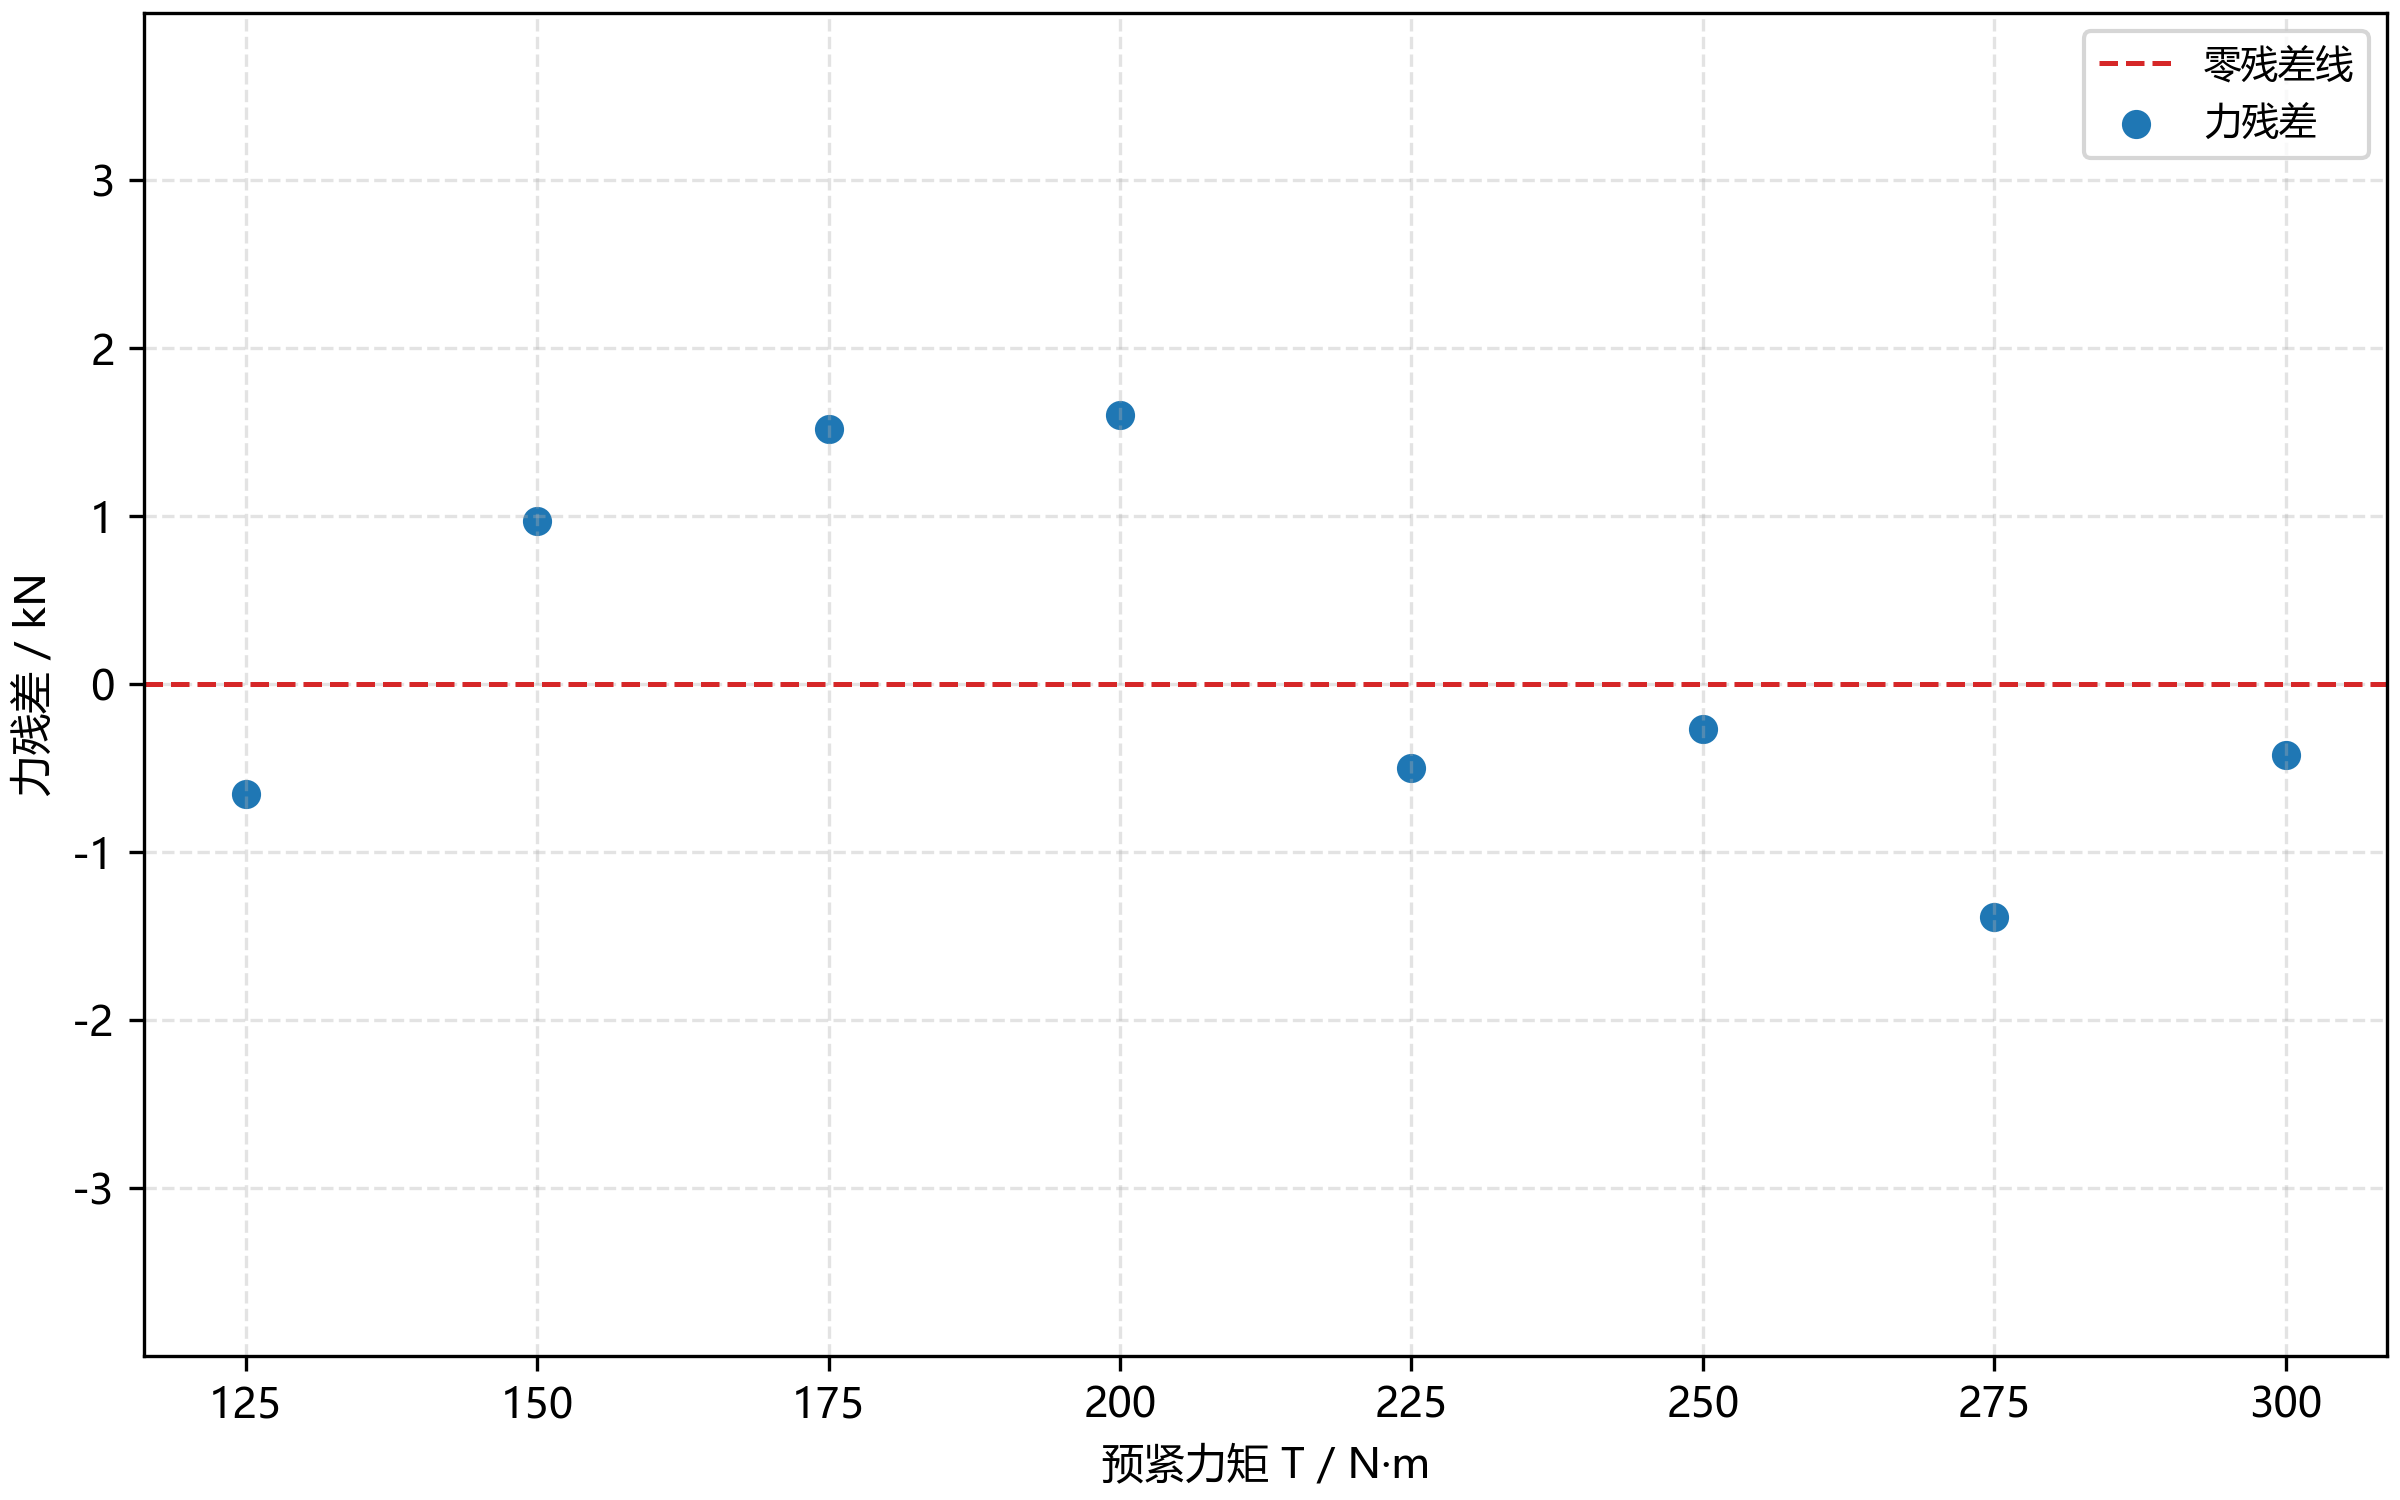
\includegraphics[width=0.85\textwidth]{outputs/figures/question1_2_rock_fixed_residuals.png}
\caption{岩石工况临界点后残差分布}
\end{figure}
得到的线性关系的拟合公式为
\begin{equation}
T=4.272P,\qquad R^2=0.9940
\end{equation}
说明直线拟合效果很好，对应残差范围约为 $[-1.384,1.599]\ \text{kN}$。残差整体围绕零残差线分布，没有出现随力矩增大而持续单调的趋势，说明在该临界点之后，线性模型能够较好描述预紧力矩与预紧力之间的关系。

对煤体工况，得到拟合直线与残差如下
\begin{figure}[H]
\centering
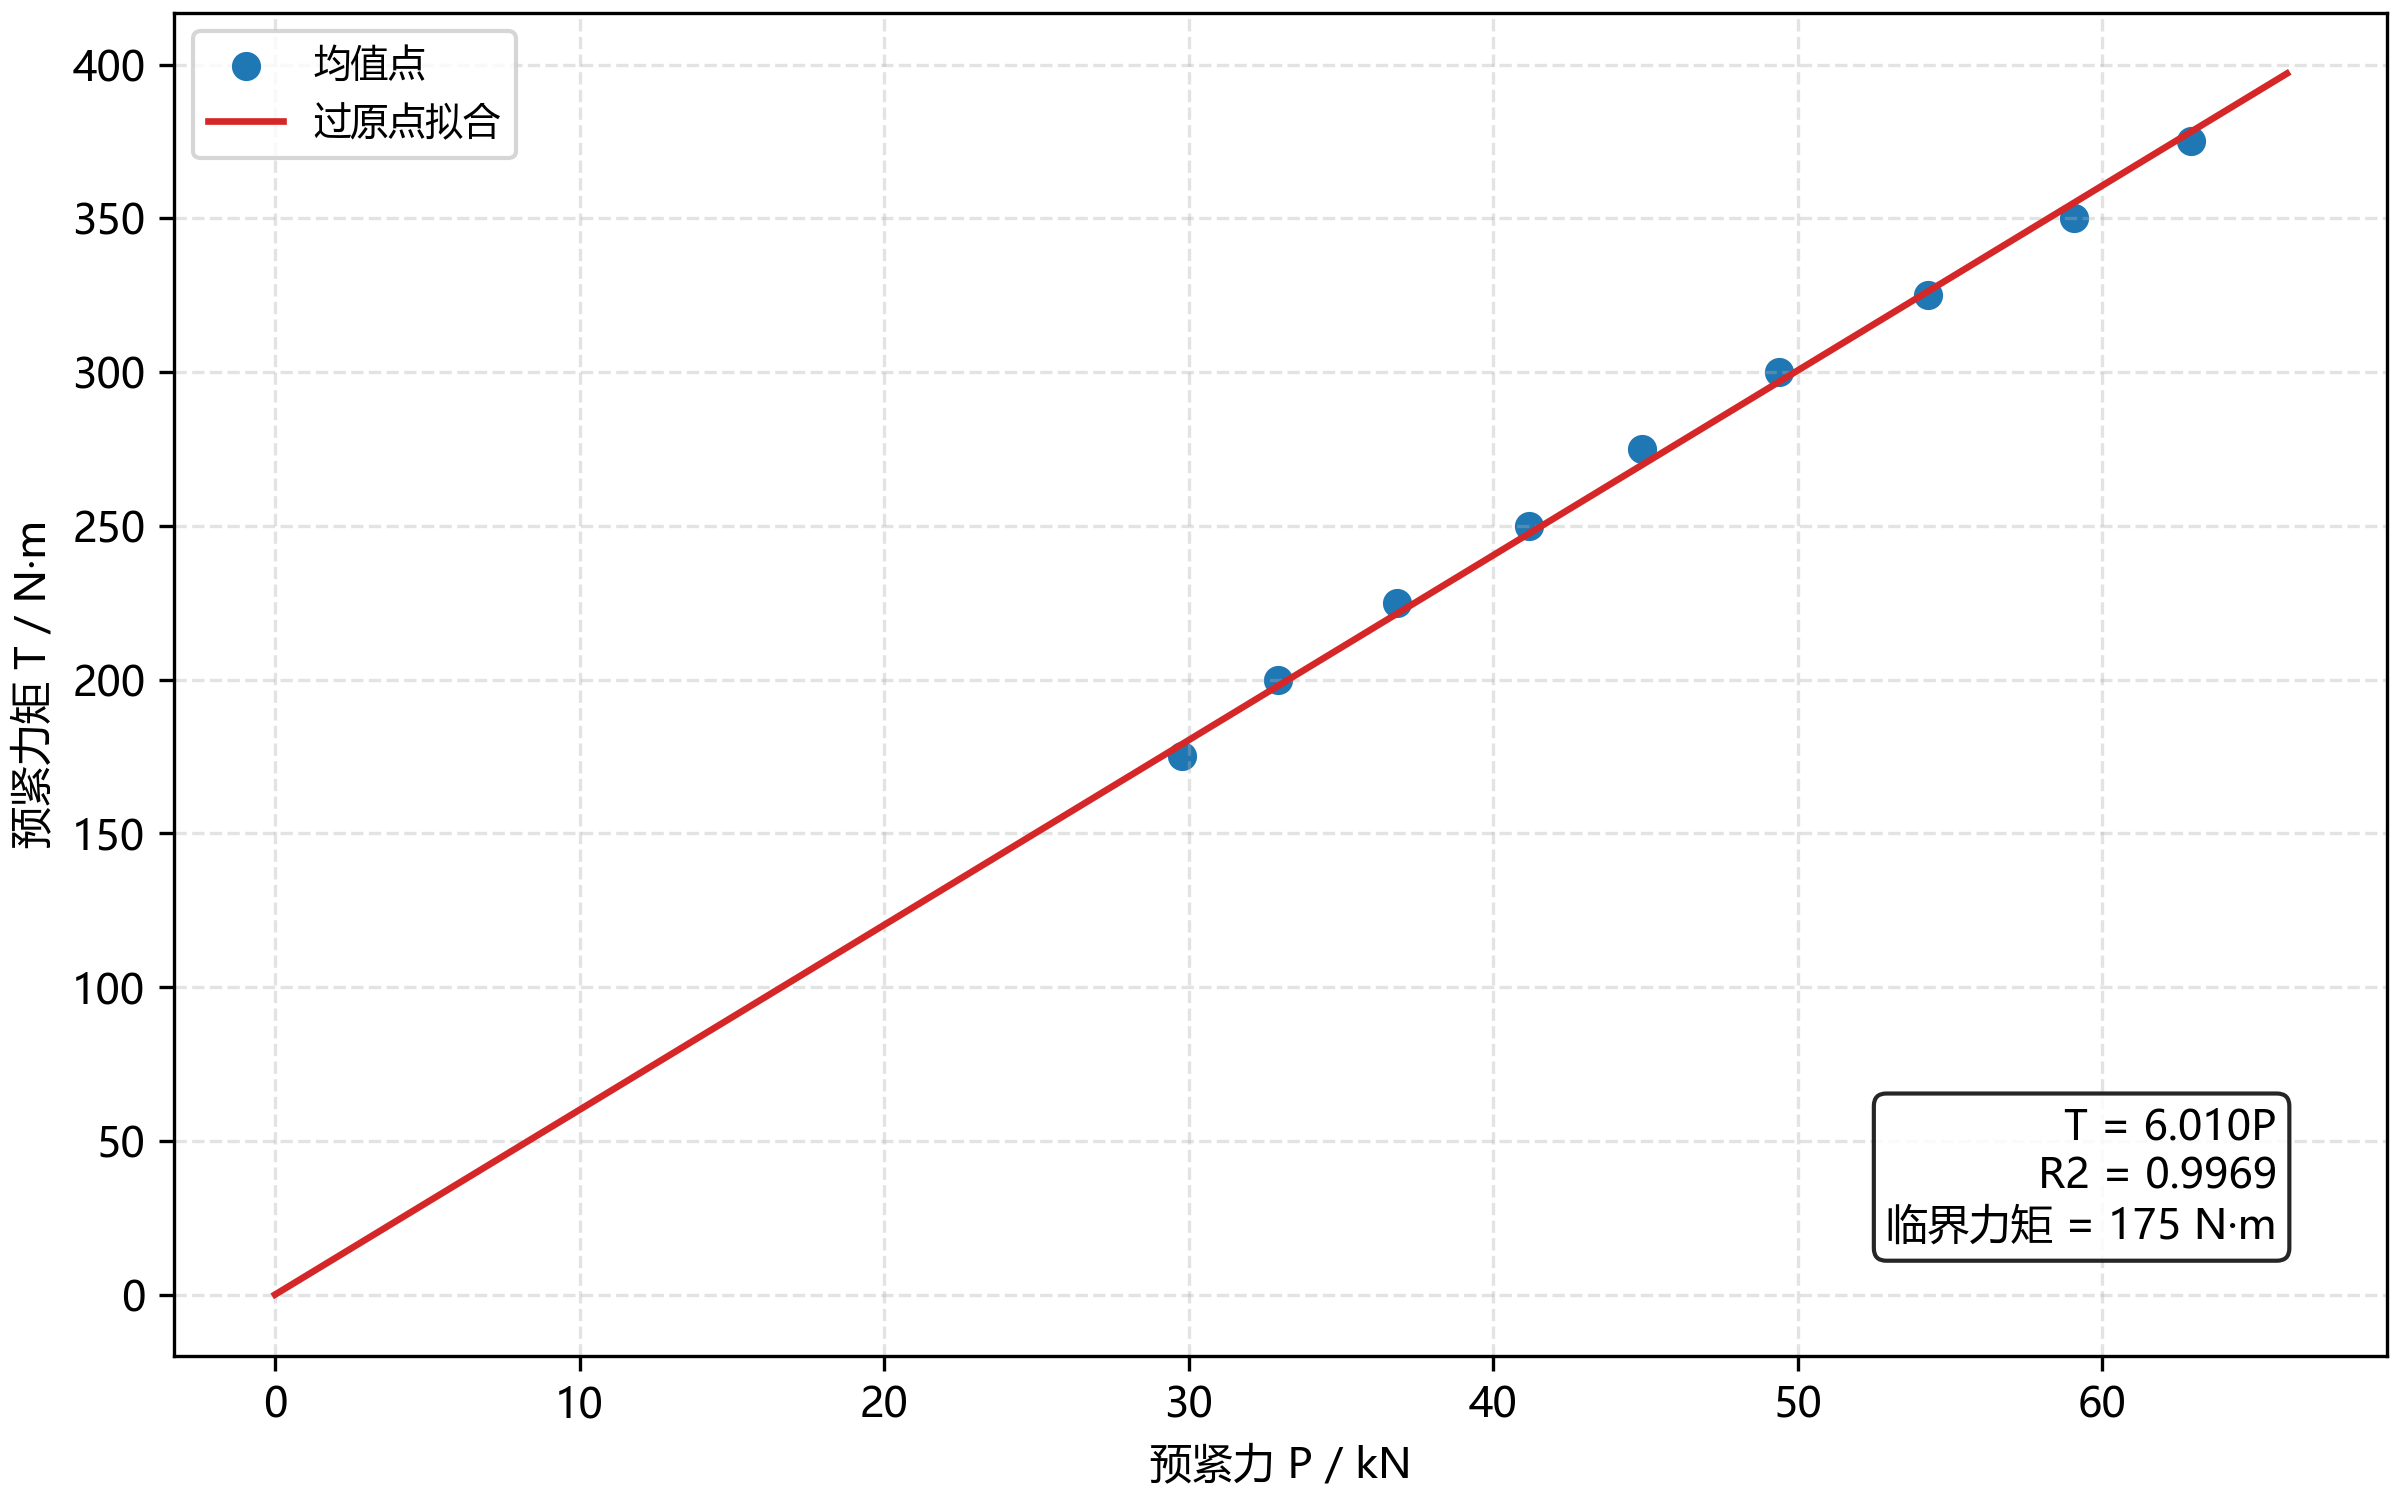
\includegraphics[width=0.85\textwidth]{outputs/figures/question1_2_coal_fixed_fit.png}
\caption{煤体工况临界点后数据拟合结果}
\end{figure}
\begin{figure}[H]
\centering
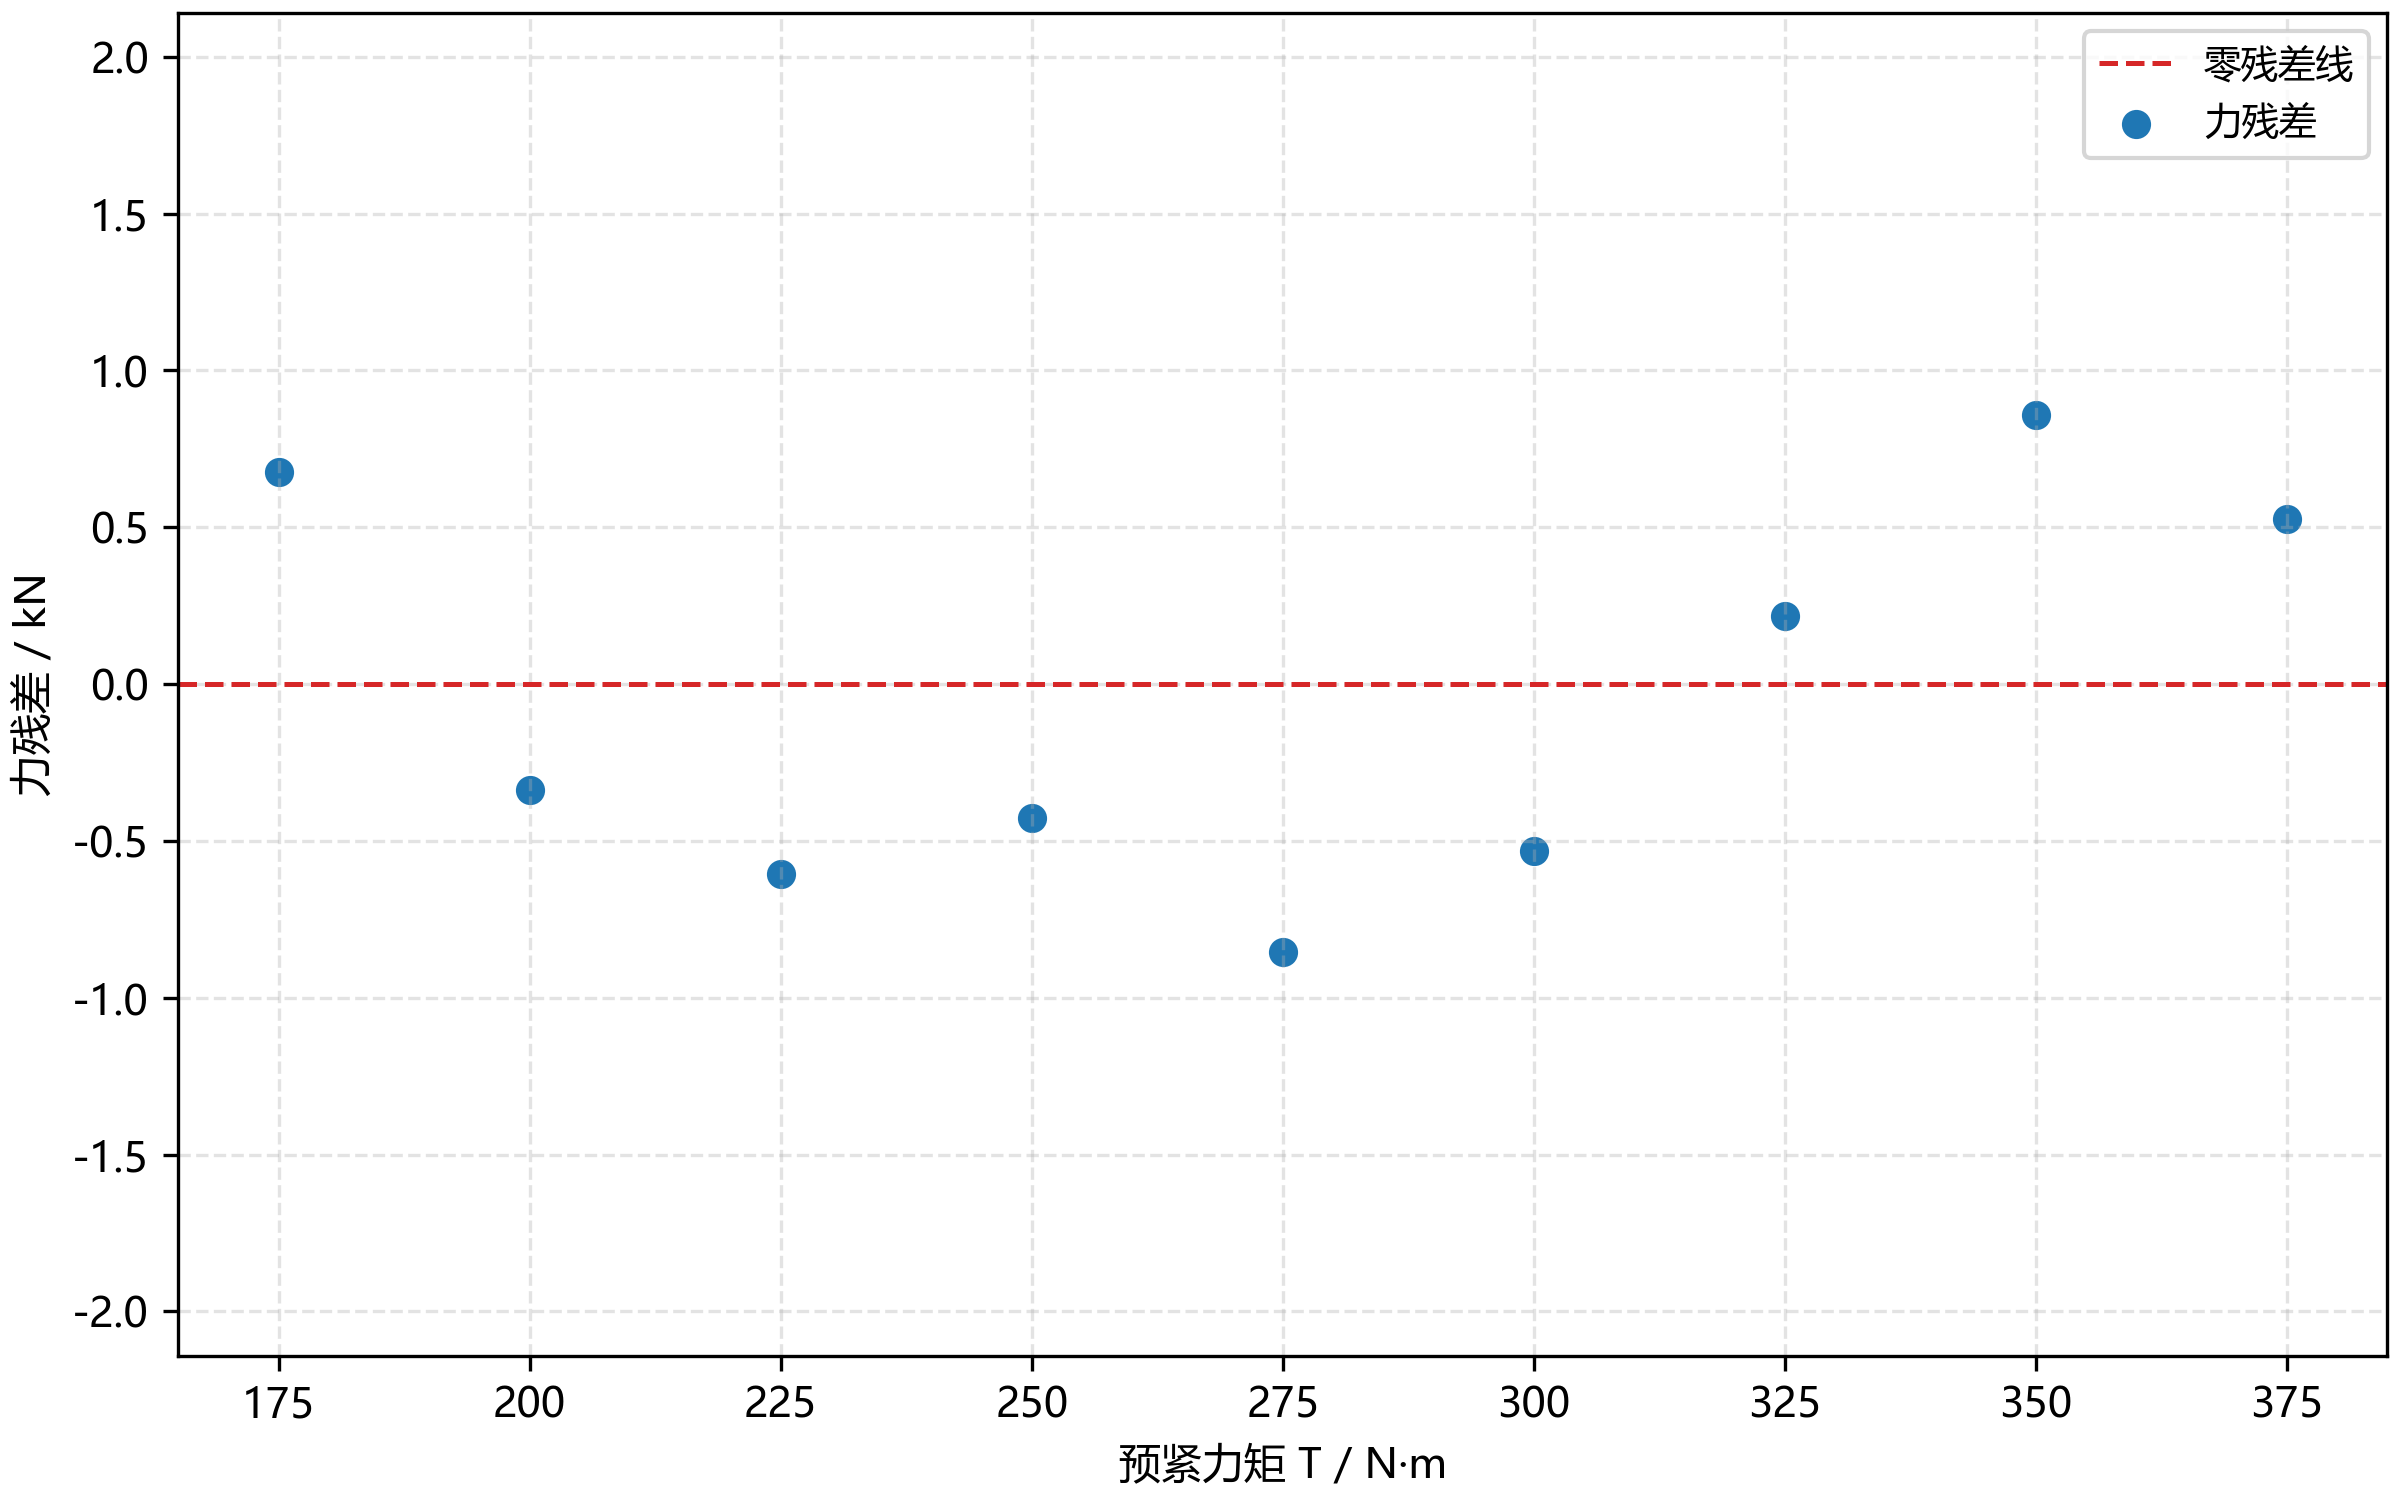
\includegraphics[width=0.85\textwidth]{outputs/figures/question1_2_coal_fixed_residuals.png}
\caption{煤体工况临界点后残差分布}
\end{figure}
得到的线性关系的拟合公式为
\begin{equation}
T=6.010P,\qquad R^2=0.9969
\end{equation}
说明直线拟合效果很好，对应残差范围约为 $[-0.855,0.856]\ \text{kN}$，残差无明显波动，说明线性模型能够较好描述预紧力矩与预紧力之间的关系。

而从实际工程角度看，与岩石工况相比，煤体工况所需临界力矩更高，这与煤体结构较软，在低力矩阶段更容易发生局部压密和接触状态调整有关，证明了我们的答案在工程上是能解释的。当预紧力矩达到较高水平后，锚杆与煤体接触状态趋于稳定，两种工况下扭矩向轴向预紧力的传递关系也符合了线性关系。

\subsection{问题二的模型建立与求解}
\subsubsection{问题2.1建模与分析}
由第一问可知，预紧力矩与预紧力有一定的关系，在这里我们利用其成线性关系的部分进行数学模型的建立。由于预紧力矩与预紧力在线性部分是成正比的，所以要找到最大允许预紧力矩$T_{max}$就是找到最大的预紧力$P_{max}$。

由附录二可知，预紧力需要满足下述约束条件：
\begin{enumerate}
    \item 锚杆强度极限：预紧力P不得超过锚杆杆体的屈服载荷$P_{yield}$，即
    \begin{equation}
        P\le P_{yield}
    \end{equation}
    \item 锚固系统极限：预紧力P不得超过锚固剂与围岩的极限粘结力$F_{bond}$，结合$F_{bond}$计算公式可得
    \begin{equation}
        P\le F_{bond}=\Pi \cdot D_{hole} \cdot L_{bond} \cdot \tau \cdot 10^{-3}(kN)
    \label{q4-lim2-raw1}
    \end{equation}
    其中$D_{hole}$为钻孔直径(mm)，$L_{bond}$为有效锚固长度(mm)，$\tau$为围岩与锚固剂界面的剪切强度(MPa)。同时剪切强度$\tau$（单位MPa）与围岩弹性模量E（单位Gpa）还满足以下关系
    \begin{equation}
        \tau=0.25E+1
    \label{q4-lim2-raw2}
    \end{equation}
    \item 围岩压陷极限：当只使用托盘时，托盘对围岩的压入深度$\delta$不能超过允许压入深度$\delta_{max}$，否则需要使用钢带。当仅使用托盘时，压入深度$\delta$可采用Winkler弹性地基模型估算，可得
    \begin{equation}
        \delta=\frac{P(1-\nu^2)h_0}{Eb^2}\le \delta_{max}
    \label{q4-lim3-raw}
    \end{equation}
\end{enumerate}
 
 结合上述三个约束，建立在给定地质和支护参数下的最大允许预紧力矩$T_{max}$的通用参数化模型就转化为下述优化问题：
 \begin{enumerate}
     \item 当仅使用托盘时
     \begin{equation}
\begin{aligned}
    \max_{T,P}\quad & T \\[1mm]
    \mathrm{s.t.}\quad
    & T = KdP,\\
    & P \leq P_{\mathrm{yield}},\\
    & P \leq
    \Pi D_{\mathrm{hole}}
    L_{\mathrm{bond}}
    (0.25E+1) \cdot 10^{-3},\\
    & P \leq
    \frac{\delta_{\max}Eb^2}
    {(1-\nu^2)h_0},\\
    & T \geq 0,\quad P \geq 0.
\end{aligned}
\label{meigangdai}
\end{equation}

\item 当可以使用钢带时，由于钢带可以分散压力从而使得压入深度减小，所以在使用钢带时可以认为围岩压陷极限的影响力相比于另外两个极限的影响时次要的，因此可以得到
\begin{equation}
\begin{aligned}
    \max_{T,P}\quad & T \\[1mm]
    \mathrm{s.t.}\quad
    & T = KdP,\\
    & P \leq P_{\mathrm{yield}},\\
    & P \leq
    \Pi D_{\mathrm{hole}}
    L_{\mathrm{bond}}
    (0.25E+1) \cdot 10^{-3},\\
    & T \geq 0,\quad P \geq 0.
\end{aligned}
\label{yougangdai}
\end{equation}
\end{enumerate}

其中，当\[P > \frac{\delta_{\max}Eb^2}{(1-\nu^2)h_0}\]时必须使用钢带

同时，由于预紧力矩与预紧力是成正比的，所以对允许的最大预紧力矩$T_{max}$的模型可以进一步转化为
\begin{enumerate}
    \item 仅使用托盘时，
    由优化问题-式~\ref{meigangdai}解得
    \begin{equation}
        T_{max}=Kd\min
    \left\{
    P_{\mathrm{yield}},
    \Pi D_{\mathrm{hole}}
    L_{\mathrm{bond}}
    (0.25E+1) \cdot 10^{-3},
    \frac{\delta_{\max}Eb^2}
    {(1-\nu^2)h_0}
    \right\}
    \label{jieguo}
    \end{equation}
    \item 当可以使用钢带时，由上述优化问题-式~\ref{yougangdai}解得
    \begin{equation}
        T_{max}=Kd\min
    \left\{
    P_{\mathrm{yield}},
    \Pi D_{\mathrm{hole}}
    L_{\mathrm{bond}}
    (0.25E+1) \cdot 10^{-3}
    \right\}
    \end{equation}
    \end{enumerate}
    
其中，当
\begin{equation}
    \frac{\delta_{\max}Eb^2}{(1-\nu^2)h_0}<\min
    \left\{
    P_{\mathrm{yield}},
    \Pi D_{\mathrm{hole}}
    L_{\mathrm{bond}}
    (0.25E+1) \cdot 10^{-3}
    \right\}
    \label{yby}
\end{equation}
时必须使用钢带。
    
从上述模型中，我们可以看出是否需要使用钢带，取决于围岩压陷极限对应的预紧力与另外两个极限对应的预紧力之间的关系，若
\[\frac{\delta_{\max}Eb^2}{(1-\nu^2)h_0}<\min
    \left\{
    P_{\mathrm{yield}},
    \Pi D_{\mathrm{hole}}
    L_{\mathrm{bond}}
    (0.25E+1) \cdot 10^{-3}
    \right\}\]
\textbf{即围岩压陷极限对应的预紧力小于另外两个极限对应的预紧力时，必须使用钢带，反之则不需要使用钢带}。

\subsubsection{问题2.2的求解}
在问题1.2中我们求出了锚杆直径为$20$mm时岩层锚杆的扭矩系数K=0.2136；煤层锚杆的扭矩系数K=0.3005。但是表4给出煤层使用的是直径$22$mm的锚杆，因此需要进一步计算此时的K值。由于问题1.1说明了直径$d$的变化会影响扭矩系数K，但我们并不清楚在实际工况下的K值会有何变化。所以考虑使用问题1.1中在理想实验下测得的不同直径$d$对应的扭矩系数K计算修正系数求解。定义煤体修正系数为煤体实际扭矩系数与理想实验扭矩系数之比，即
\begin{equation}
\lambda_c=\frac{K_{20}^{(c)}}{K_{20}^{(0)}}
\end{equation}
代入$K_{22}^{(0)}$得到表4所给煤层工况下对应的K值为0.3117。

在问题2.1中，我们对最大预紧力矩进行了建模，并讨论了其需要使用钢带的情况，在这一问中，我们只需要将对应的数据代入到上述式~\ref{jieguo}中计算最大预紧力矩，再通过式~\ref{yby}来判断是否需要钢带即可。

将工况A：岩层锚杆的相关数据代入上述式子中可以计算出锚杆强度极限对应预紧力为170 kN，锚固系统极限对应的预紧力为334.265 kN，围岩压陷极限对应的预紧力为400kN，所以\textbf{最大的预紧力$P_{max}=$170kN},\textbf{最大允许预紧力矩$T_{max}=$726.24{N$\cdot$m}}。由于围岩压陷极限对应的预紧力是大于前面求得的最大的预紧力的，所以\textbf{不需要使用钢带}。

将工况B：煤层锚杆的相关数据代入上述式子中可以计算出锚杆强度极限对应预紧力为205 kN，锚固系统极限对应的预紧力为169.646 kN，围岩压陷极限对应的预紧力为123.077kN，所以\textbf{在仅使用托盘时最大的预紧力$P_{max}=$123.077kN},\textbf{最大允许预紧力矩$T_{max}=$843.938N$\cdot$m}；\textbf{在允许使用钢带时最大的预紧力$P_{max}=$169.646kN},\textbf{最大允许预紧力矩$T_{max}=$1163.263N$\cdot$m}。同时由于围岩压陷极限对应的预紧力是小于另外两个极限对应的预紧力的，所以\textbf{需要使用钢带}。

\subsection{问题三的模型建立与求解}

\subsubsection{问题3.1建模与分析}
根据附录三可知，锚杆螺纹段同时承受以下三种应力的联合作用：
\begin{enumerate}
    \item 轴向拉应力$\sigma_t$：由预紧力P引起：
    \begin{equation}
        \sigma_t=\frac{P}{A_e}=\frac{T}{KdA_e}
    \end{equation}
    \item 弯曲应力$\sigma_b$：由偏心距e引起的附加弯矩$M=p\cdot e$导致：
    \begin{equation}
        \sigma_b=\frac{P\cdot e}{W_b}=\frac{T\cdot e}{KdW_b}
    \end{equation}
    \item 扭转剪应力$\tau$：由施工拧紧过程中的螺纹段有效扭矩$T_s=K_S\cdot T$引起：
    \begin{equation}
        \tau=\frac{K_S\cdot T}{W_t}
    \end{equation}
\end{enumerate}
这三种应力的叠加可能导致锚杆在螺纹根部发生齐根断裂。工程上常采用VonMises等效应力准
则进行判断，要求等效应力$\sigma_{eq}$不超过材料的许用应力[$\sigma$]：
\begin{equation}
    \sigma_{eq}=\sqrt{(\sigma_t+\sigma_b)^2+3\tau^2}\le [\sigma]
    \label{panduan}
\end{equation}
其中$A_e$为有效截面积，$W_b$为抗弯截面系数，$W_t$为抗扭截面系数，许用应力[$\sigma$]=500MPa。

从上述式子可以看出，在偏心受力下，预紧力矩要满足使等效应力不超过材料的许用应力，所以最大允许预紧力矩$T_max$就是当等效应力等于材料的许用应力时的预紧力矩。

由附录一可知
\begin{equation}
    A_e=\frac{\pi d_e^2}{4}
\end{equation}
\begin{equation}
    W_b=\frac{\pi d_e^3}{32}
\end{equation}
\begin{equation}
    W_t=\frac{\pi d_e^3}{16}
\end{equation}

将上述式子代入式~\ref{panduan}中即可得到预紧力矩T的最大值：
\begin{equation}
    T_{max}=\frac{Kd\Pi d_e^3[\sigma]}{4\sqrt{(d_e+8e)^2+48K_s^2K^2d^2}} \cdot 10^{-3}(N\cdot m)
\label{q4-lim4-raw}
\end{equation}

下面对模型的适用性与局限性进行分析：

适用性：
\begin{enumerate}
    \item 可用于研究偏心距对最大预紧力矩的影响:从模型结果可以看出允许最大预紧力矩$T_{max}$随偏心距 e 单调减小；当偏心距较大时，其变化近似呈反比例规律，符合材料力学中偏心拉伸构件的基本受力规律。
    \item 工程实用性：其应力叠加在弹性阶段直接采用$\sigma_t+\sigma_b$具有合理性且计算简便，同时采用Vonmises等效应力准则进行判断也让它更适用于工程预测。
    \item 施工初步方案分析：其参数具有明确意义且便于测量，同时该模型的计算量较小，适用于施工初期进行初步分析时使用。
\end{enumerate}

局限性：
\begin{enumerate}
    \item 名义应力的假设：这个模型中计算都是采用的名义应力，而在实际工程中，由于螺纹根部截面突变会导致应力集中，所以实际应力大小可能会高于名义最大应力，导致模型高估了锚杆的实际承载能力。
    \item 偏心距固定取值：在这个模型中，偏心矩使用的是固定值，但在实际工程中随着预紧力增加，托盘，围岩等的状态可能会不断变化，导致偏心距在变化，使得偏心距是预紧力或者预紧力矩的函数。
    \item 扭转系数被视为常数：在实际工程中，扭转系数会受实际影响而发生变化，导致这个最大应力会发生变化，所以不适用于全过程的预测。
    \item 接触面非线性：该模型忽略了托盘与岩体的接触面的实际情况，导致计算结果与实际结果会有较大偏差。
\end{enumerate}

\subsubsection{问题3.2建模与分析}
附录二所示的工程约束大多建立在理想情况下，而实际工程中由于偏心距e的存在，不仅会使锚杆螺纹段产生附加弯曲应力，还可能改变托盘与围岩之间的压力分布，因此这些约束会出现一定的偏差，下面对这个约束模型进行修正。

\begin{enumerate}
    \item 锚杆强度极限：受轴向拉应力，弯曲应力和扭转剪应力三种应力的影响，预紧力P可能达不到锚杆杆体的屈服载荷$P_{yield}$,而是由于三种应力的叠加导致锚杆在螺纹根部发生齐根断裂，因此此处需要修改为
    \begin{equation}
        p\le \min
    \left\{
    P_{\mathrm{yield}},
    \frac{\Pi d_e^3[\sigma]}{4\sqrt{(d_e+8e)^2+48K_s^2K^2d^2}} \cdot 10^{-3}
    \right\}
    \end{equation}
    \item 锚固系统约束：这一约束主要来自2锚固剂与围岩的极限粘结力$F_{bond}$，由于题目未给出偏心弯矩作用下锚固界面的剥离强度和非均匀剪应力分布参数，本文在一阶近似中保留原锚固极限公式不变。
    \item 围岩压陷极限：偏心距e的存在使得托盘不仅受到轴向压力P还会受到由偏心距e引起的附加弯矩M=Pe，假设托盘为边长为b的方形，在托盘与围岩保持完全接触、接触压力沿偏心方向线性变化的条件下，接触压强可表示为\cite{ivan2010eccentric}
    \begin{equation}
        q_i
    =
    \frac{P}{A}
    \left(
        1+
        \frac{x_i e_x}{i_y^2}
        +
        \frac{y_i e_y}{i_x^2}
    \right)
    \end{equation}
    其中A为承压面积，$e_x,e_y$为两个方向上的偏心距，$x_i,y_i$为计算点相对于承压面形心的坐标，$i_x,i_y$为承压面关于相应轴的回转半径。

    为了简化计算，我们假设预紧力只往一个方向偏心，即$e_x=e,e_y=0$，将式子进一步化简为
    \begin{equation}
        q(x)
    =
    \frac{P}{A}
    \left(
        1+
        \frac{x e}{i_y^2}
    \right)
    \end{equation}
    由于托盘是边长为b的方形，所以承压面积\[A=b^2\]关于 y 轴的截面惯性矩为\[I_y=\frac{b^4}{12}\]回转半径满足\[i_y^2=\frac{I_y}{A}=\frac{b^2}{12}\]
    将上述式子进行整理，得到
    \begin{equation}
        q(x)
    =
    \frac{P}{b^2}
    \left(
        1+
        \frac{12x e}{b^2}
    \right),
    \end{equation}
    不难看出，最大接触压强位于接触边缘，此时$x=\frac{b}{2}$,所以最大压强可表示为
    \begin{equation}
        q(x)
    =
    \frac{P}{b^2}
    \left(
        1+
        \frac{6e}{b}
    \right),
    \end{equation}
    其中偏心距e应满足\[0\le e\le \frac{b}{6}\]否则托盘一侧会出现脱离接触，当前线性压强分布模型不再成立。
    由附录二可以看出，压入深度$\delta$与接触压强成正比，所以该约束应修正为
    \begin{equation}
        \delta=\frac{P(1+\frac{6e}{b})(1-\nu^2)h_0}{Eb^2}\le \delta_{max}
    \end{equation}
    整理可得
    \begin{equation}
        P\le\frac{\delta_{\max}Eb^2}{(1+\frac{6e}{b})(1-\nu^2)h_0},
    \end{equation}
    
\end{enumerate}
结合上述约束修正和问题二的建模思路，我们不难得出此时最大允许预紧力矩$T_{max}(e)$的数学表达式为：
\begin{enumerate}
    \item 仅使用托盘时
    \begin{equation}
    \begin{aligned}
        T_{max}(e)=&Kd\min
    \left\{
    P_{\mathrm{yield}},
    \frac{\Pi d_e^3[\sigma]\cdot 10^{-3}}{4\sqrt{(d_e+8e)^2+48K_s^2K^2d^2}} ,
   F_{bond},
    \frac{\delta_{\max}Eb^2}{(1+\frac{6e}{b})(1-\nu^2)h_0}
    \right\}\\
    &\qquad\qquad
    0\le e\le\frac{b}{6}
    \end{aligned}
    \end{equation}
    其中\[F_{bond}=\Pi D_{\mathrm{hole}}
    L_{\mathrm{bond}}
    (0.25E+1) \cdot 10^{-3}\]
    \item 可以使用钢带时
     \begin{equation}
     \begin{aligned}
        T_{max}(e)=&Kd\min
    \left\{
    P_{\mathrm{yield}},
    \frac{\Pi d_e^3[\sigma]\cdot 10^{-3}}{4\sqrt{(d_e+8e)^2+48K_s^2K^2d^2}} ,
   \Pi D_{\mathrm{hole}}
    L_{\mathrm{bond}}
    (0.25E+1) \cdot 10^{-3}
    \right\}\\
    &\qquad\qquad
    0\le e\le\frac{b}{6}
    \end{aligned}
     \end{equation}
    其中，当\[\frac{\delta_{\max}Eb^2}{(1+\frac{6e}{b})(1-\nu^2)h_0}\le \min
    \left\{
    P_{\mathrm{yield}},
    \frac{\Pi d_e^3[\sigma]\cdot 10^{-3}}{4\sqrt{(d_e+8e)^2+48K_s^2K^2d^2}} ,
   \Pi D_{\mathrm{hole}}
    L_{\mathrm{bond}}
    (0.25E+1)10^{-3}
    \right\}\]时，必须使用钢带。
\end{enumerate}

接下来对仅使用托盘的情况，参照问题二所用的表四提供的参数以及附录三提供的参数进行数值验证。
我们将参数代入上面建立的模型中，对偏心距以0.1mm为步长，从0到$\frac{b}{6}$取不同值再进行作图,分别得出岩层锚杆和煤层锚杆最大预紧力矩$T_{max}(e)$随e变化曲线图如下所示



\subsection{问题四的模型建立与求解}
\subsubsection{模型建立}
由附录1可知：f为普氏系数，表征岩石坚固程度的经验指标，数值越大岩石越坚硬，其与单轴抗压强度$\sigma_c$（单位:Mpa）有如下关系：
\begin{equation}
    f=\frac{\sigma_c}{10}
\label{q4-fandc}
\end{equation}
即：
\begin{equation}
    \sigma_c=10f
\end{equation}
故现在转为寻找$\sigma_c$与弹性模量E的关系。通过查阅文献资料可知，在面对单个同一岩体时，其弹性模量E与其单轴抗压强度$\sigma_c$呈正相关\cite{lin2017ucs}，使用Deere的岩石分类思想\cite{deere1966engineering}，我们可以有如下近似关系：
\begin{equation}
    E_R=M_R\sigma_c
\end{equation}
其中，$E_R$为完整弹性模量,而$M_R=\frac{E}{\sigma_c}$称为模量比，但是不同岩石的模量比$M_R$并不相同，在Deere-Miller分类中，多数具有较完整、互锁结构的岩石落在:
\begin{equation*}
    200\le M_R \le500
\end{equation*}
范围内，平均参考线通常取$M_R=300$作为基准值\cite{deere1966engineering}，本文故也采用这一基准值用于模型构建。
此外考虑到实际情况下，围岩不能保证完全完整，故取完整性折减系数$\eta\in(0,1]$来获得实际弹性模量E与单轴抗压强度$\sigma_c$的关系：
\begin{equation}
    E=\eta E_R=\eta M_R\sigma_c
\label{q4-Eandc}
\end{equation}
将式~\ref{q4-fandc}带入式~\ref{q4-Eandc}，可得：
\begin{equation}
    E=10\eta M_Rf
\label{q4-Eandf-raw}
\end{equation}
但此时弹性模量E的单位为MPa，考虑到后续约束中E使用的单位为GPa，我们对式~\ref{q4-Eandf-raw}进行单位转换：
\begin{equation}
    E=0.01\eta M_Rf ~(Gpa)
\label{q4-Eandf}
\end{equation}
则我们可以根据各失效约束得出下列关系：
\begin{enumerate}
    \item 对于锚杆强度极限约束，其与只与材料有关，则预紧力应满足：
    \begin{equation}
        P\le P_{yield}
    \label{q4-lim1-raw}
    \end{equation}
    可知该项约束与普氏系数f无关，是上界约束。

    \item 对于锚固系统极限约束，问题二建模过程已经给出了对应约束，即式~\ref{q4-lim2-raw1}、式~\ref{q4-lim2-raw2}，结合式~\ref{q4-Eandf}，带入式~\ref{q4-lim2-raw1}整理可得：
    \begin{equation}
        P\le \Pi\cdot D_{hole}\cdot L_{bond}\cdot (0.25\eta M_Rf\cdot 10^{-2}+1.0)\cdot 10^{-3}
    \label{q4-lim2}
    \end{equation}
    可见该约束下，P的上界随f的增大而增大。

    \item 对于围岩压陷极限约束，同样的问题二已经给出了约束关系式~\ref{q4-lim3-raw}，将式~\ref{q4-Eandf}带入可得：
    \begin{equation}
        P\le \frac{0.01\delta_{max}\cdot \eta\cdot M_Rf\cdot b^2}{(1-\nu^2)h_o}
    \label{q4-lim3}
    \end{equation}
    可见该约束下，P的上界也是随着f的增大而增大。
    
\end{enumerate}
至此我们得到了三项约束关系，原问题则转换为如下优化问题：
\begin{equation}
\begin{aligned}
    \max_{T,P}\quad & T \\[1mm]
    \mathrm{s.t.}\quad
    & T=Kd\cdot P ,\\
    & P\le P_{yield},\\
    & P\le \Pi\cdot D_{hole}\cdot L_{bond}\cdot (0.25\eta M_Rf\cdot 10^{-2}+1.0)\cdot 10^{-3},\\
    & P\le \frac{0.01\delta_{max}\cdot \eta\cdot M_Rf\cdot b^2}{(1-\nu^2)h_o}.
\end{aligned}
\end{equation}
记三项约束等号取值分别为：
\begin{equation*}
\begin{aligned}
    & P_1=P_{yield},\\
    & P_2=\Pi\cdot D_{hole}\cdot L_{bond}\cdot (0.25\eta M_Rf\cdot 10^{-2}+1.0)\cdot 10^{-3},\\
    & P_3=\frac{0.01\delta_{max}\cdot \eta\cdot M_Rf\cdot b^2}{(1-\nu^2)h_o},\\
\end{aligned}
\end{equation*}

则得\begin{equation}
    T_{max}=Kd\cdot \min(P_1,P_2,P_3)
\end{equation}
可取使支护效果较优而不触发任何失效约束的预紧力矩 :
\begin{equation}
    T_{opt}=\gamma T_{max}=\gamma Kd\cdot \min(P_1,P_2,P_3)
\label{q4-Topt}
\end{equation}
其中，$\gamma\in(0,1)$为安全裕度系数，用于确保$T_{opt}$能距离某个主控失效约束边界上仍有裕度，以确保模型不触发任何失效约束。在后续有效性、可靠性验证中，我们采用$\gamma=0.8$的安全裕度系数来证明模型在大部分情况下是有效且可靠的。

\subsubsection{失效分析}
已知$P_1$为上界约束，则优先考虑$P_2$与$P_3$之间的竞争程度，故我们对其取竞争约束比，记为：
\begin{equation}
\begin{split}
    R_{23}(f) &= \frac{P_2}{P_3} 
         = \frac{\Pi\cdot D_{hole}\cdot L_{bond}\cdot (0.25\eta M_Rf\cdot 10^{-2}+1.0)\cdot 10^{-3}}{\frac{0.01\delta_{max}\cdot \eta\cdot M_Rf\cdot b^2}{(1-\nu^2)h_o}} \\
        &=\kappa_{23}\cdot(\alpha_\tau+\frac{1}{f})
\end{split}
\end{equation}
其中$\kappa_{23}=\frac{\Pi\cdot D_{hole}\cdot L_{bond}\cdot (1-\nu^2)h_0}{10\cdot \delta_{max}\cdot \eta M_R\cdot b^2}$为比例系数，$\alpha_\tau=0.25\eta M_R\cdot 10^{-2}$为剪切强度转换系数。
当$R_{23}(f)>1$时，有$P_2>P_3$，说明二者之间由$P_3$起控制作用；当$R_{23}(f)<1$时，有$P_2<P_3$，说明二者之间由$P_2$起控制作用；当$R_{23}(f)=1$时,两种失效约束达到临界状态；由此我们可作出下列分析：
\begin{enumerate}
    \item 当$f<3$，即松软围岩性质时，$R_{23}(f)>1$，且$P_2<P_{yield}$，故主控失效约束为$P_3$，即\textbf{围岩压陷极限}，此时锚杆强度足够，锚固剂粘结强度也足够，但是围岩不能承受较大预紧力，若要解决，办法之一是添加钢带。

    \item 当$3\le f < 6$，即中等强度围岩性质时，容易出现$R_{23}(f)<1$，且$P_3<P_{yield}$，故此时主控失效约束主要为$P_2$，即\textbf{锚固系统极限}，此时围岩能承受一定预紧力，锚杆强度也仍可支撑，但是锚固剂粘结力有限，故成为主控失效约束，若要解决，办法之一是改用高强度锚固剂。

    \item 当$f\ge 6$，即坚硬围岩性质时，由上述分析知：$P_2$与$P_3$都随着f的增大而增大，此时主要情况为$P_2>P_1$、$P_3>P_1$，则主控失效约束为$P_1$，即\textbf{锚杆强度极限}，此时围岩和锚固剂都能支撑强大预紧力，但是锚杆自身强度不足以支撑巨大预紧力，故成为主控失效约束，若要解决，办法之一是使用高强度锚杆。
    
\end{enumerate}

\subsubsection{有效性与可靠性验证}
对于有效性与可靠性的验证，我们选择使用附件表4中提供的工况数据进行数值验证，采用满足上界的方法，即依据模型，根据式~\ref{q4-Topt}，计算使支护效果较优而不触发任何失效约束的预紧力矩$T_{opt}$，同时也计算原约束“锚杆强度极限”、“锚固系统极限”、“围岩压陷极限”，并通过比较数值来进行验证。
\begin{enumerate}
    \item 对于有效性验证，在设计上，我们设计了$T_{opt}=\gamma \min(T_1,T_2,T_3)$，其中$T_1,T_2,T_3$分别对应三种约束失效时对应的预紧力矩，而由于$\gamma \in (0,1)$，因此理论上必有:
    \begin{equation*}
        T_{opt}<T_i(f),\quad i=1,2,3
    \end{equation*}
    因此模型是在实现支护效果较优而不触发任何失效约束上是有效的，下列图示也能证明其有效性。
    
    将数据带入，得到的结果如下，图示可见，在$0<f\le10$区间，$T_{opt}$线始终位于失效边界下方，说明模型所得$T_{opt}$能够满足约束条件与安全裕度的情况下取较大值，进而有尽可能好的支护效果，由此说明我们的模型是有效的。

    \item 对于可靠性验证，我们采用扰动分析的方法，即在有效性分析得到$T_{opt}$后固定$T_{opt}$，然后在同一组环境和参数下，对参数进行扰动调整，浮动比例为10\%与20\%，并分别进行单参数扰动和多参数扰动，计算安全率。
    
    最终计算结果如下，图示可见，单参数扰动下工况A环境中，对于全部扰动情形，模型能够实现支护效果较优而不触发任何失效约束，工况B环境中，模型能够保证在10\%以内的扰动条件下完美实现要求，在20\%以内的扰动条件下，大部分扰动发生了都仍能实现要求；而多参数扰动，图示可见，即使是20\%的扰动，无论是工况A还是工况B都还能有一个较为优秀的安全率表现。
\end{enumerate}

%%%%%评价%%%%%
\section{模型评价}
\subsection{模型的优点}

\subsection{模型的缺点}

%%%%%总结%%%%%
\section{总结}

%%%%%参考文献%%%%%
\begin{thebibliography}{99}   % 99 是最大编号宽度
\bibitem{tran2026nut}
Tran V T, Nguyen H L.
Experimental investigation and reliability-based optimization of the nut factor in bolted joints considering friction coefficient, surface roughness and material hardness[J].
PLOS ONE, 2026, 21(6): e0351082.
DOI: 10.1371/journal.pone.0351082.

\bibitem{GBT1231_2024}
国家市场监督管理总局，国家标准化管理委员会.
钢结构用高强度大六角头螺栓连接副：GB/T 1231--2024[S].
北京：中国标准出版社，2024.

\bibitem{ivan2010eccentric}
IVAN A.
Pressures Distribution for Eccentrically Loaded Rectangular
Footings on Elastic Soils[C]//
Mathematical Models for Engineering Science.
2010: 213--216.

\bibitem{lin2017ucs}
林斌，徐冬.
不同岩性岩石的单轴抗压强度与弹性模量关系[J].
煤矿安全，2017，48(3)：160--162，166.
DOI: 10.13347/j.cnki.mkaq.2017.03.043.

\bibitem{deere1966engineering}
DEERE D U, MILLER R P.
Engineering Classification and Index Properties for Intact Rock[R].
Albuquerque: Air Force Weapons Laboratory, 1966.

\end{thebibliography}

\section*{附录}
\appendix

\section{文件清单}

\noindent{支撑材料的文件列表清单：}
\begin{enumerate}
    \item 
    \item 
    \item 
    \item 
\end{enumerate}

\section{代码}
\noindent{问题一代码}
\lstinputlisting[language=Python]{}

\end{document}